\documentclass{scrartcl}
\usepackage[utf8]{inputenc}
\usepackage{hyperref}
\usepackage{url}
\usepackage{natbib}
\usepackage{graphicx}
\usepackage{subfig}
\usepackage{verbatim}
\usepackage{cleveref} % this must be the last package to be loaded
\usepackage{bookmark}
\usepackage{float}


\newcommand{\emailaddr}[1]{\href{mailto:#1}{\texttt{#1}}}

\title{\LARGE
    Liar's Poker
}

\author{
    Francesco Buda \\ \emailaddr{francesco.buda3@studio.unibo.it}
    \and
    Emanuele Sanchi \\ \emailaddr{emanuele.sanchi@studio.unibo.it}
    \and
    Tommaso Severi \\ \emailaddr{tommaso.severi2@studio.unibo.it}
}

\date{February 2025}

\begin{document}

\maketitle

\begin{abstract}
This report presents the design and development of a distributed game application for playing Liar's 
Poker. It outlines all phases of the project, from the initial concept through to the final 
implementation, highlighting the evolution of the system as it was shaped to meet the specific 
demands of a distributed environment. The game logic adheres to the rules described in 
\cite{gamerules}, with adaptations made to support distributed execution.

The system architecture follows a client-server model and relies on the MQTT protocol to facilitate 
communication between components. The report provides an in-depth discussion of the design decisions 
taken throughout the project, along with detailed insights into the implementation process. Testing 
strategies are also described, focusing on both functionality and system robustness.

Particular attention is given to fault tolerance, demonstrating how the application manages client 
disconnections and server failures. The application is developed in Python, leveraging the Paho MQTT 
library to implement reliable and efficient messaging and the NiceGUI library to create a 
user-friendly web interface.
\end{abstract}

\clearpage

\tableofcontents

\clearpage

\begin{comment}

\end{comment}
\section{Concept}\label{concept}
This project aims to develop a web-based game application for playing Liar's Poker, a fun and engaging
card game centred around deception and bluffing. Inspired by traditional poker, Liar's Poker is played
with a standard deck of cards and is suitable for two or more players. Our application will provide web interface
where users can enjoy the game with others in real-time.

\subsection{Game Rules}\label{game-rules}
Liar's Poker is played with a standard deck of cards without any joker. Each player starts with one
card. A round starts with someone naming a poker combination. The turn rotate clockwise and each
next player has a choice:
\begin{itemize}
      \item \textbf{Rise the stakes}\par
            Name a higher poker combination than the one named by the previous player that
            they believe is present in the combined cards of all players.
      \item \textbf{Call bullsh*t} \par
            Call bullsh*t on the previous player's combination if the player thinks the previous
            player is bluffing or mistaken.
\end{itemize}
When someone calls bullsh*t, all players reveal their cards and the presence of the contested poker
hand is verified. If the hand is present, the player who called bullsh*t loses the round; else, the
player who named this poker hand loses the round.

The loser starts all subsequent rounds with one extra card, and names the first combination in the
next round. If someone loses when they have 5 cards, they are kicked from the game.
The last person remaining in the game is the winner.

\subsection{Questions and Answers}\label{questions-and-answers}
\begin{itemize}
      \item \textbf{Question:} \emph{How do users interact with the system?}\par
            \textbf{Answer:} Users can access the application through a web browser.
      \item \textbf{Question:} \emph{What happens if one player disconnect during the game?}\par
            \textbf{Answer:} The game will pause until the player reconnects. If the player does not
            reconnect within a certain time frame, they will be kicked from the game.
      \item \textbf{Question:} \emph{What happens if the server dies during the game?}\par
            \textbf{Answer:} The application goes on, but the game is lost. The players will be
            redirected to the lobby screen and can choose to play another game or leave the lobby.
      \item \textbf{Question:} \emph{Does the system need to store player's data?}\par
            \textbf{Answer:} The system doesn't need to store data, as the player does not need to
            create an account.
\end{itemize}

\subsection{Usage Scenarios}\label{usage-scenarios}
This section describes the typical usage scenario of a group of friends playing Liar's Poker on our
platform.
\begin{enumerate}
      \item \textbf{Name choice}\par
            Each player chooses a nickname to use during the game.
      \item \textbf{Lobby creation}\par
            One user creates a new lobby and shares the access code with friends.
      \item \textbf{Joining the lobby}\par
            Other users join the lobby by entering the code.
      \item \textbf{Gameplay}\par
            Each player receive one card and then the game starts. The game proceeds as described in
            the rules. When the player wants to rise the stakes, he can choose from the possible
            combinations (non-valid combinations will be disabled), if the combination needs some
            specific rank or suit to be declared, the player will be provided with a list of possible
            ones to choose from.
      \item \textbf{Elimination}\par
            When a player loses, they are eliminated from the game.
      \item \textbf{End of the game}\par
            When the game ends the winner is declared and players will be redirected to the lobby page
            where they can choose to play another game or leave the lobby.
\end{enumerate}

The figure \ref{fig:use-case-diagrams} shows the use case diagrams for the application.

\begin{figure}
      \centering
      \subfloat[Home and Lobby Selection]{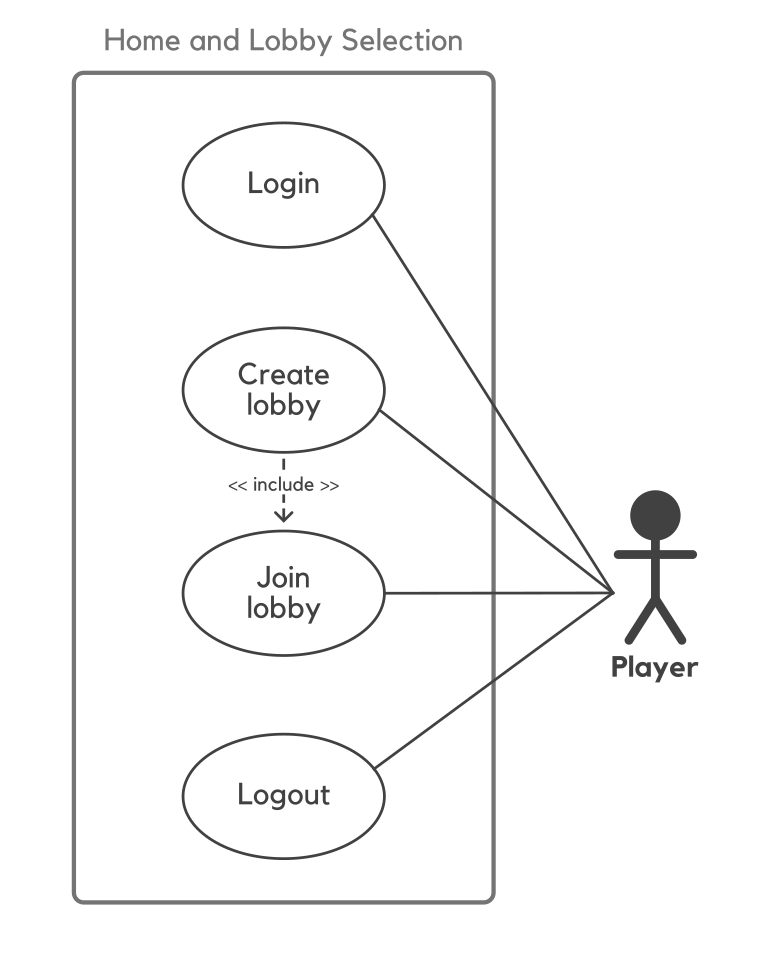
\includegraphics[width=0.5\textwidth]{figures/homeLobbyUseCase.png}}
      \hfill
      \subfloat[Lobby]{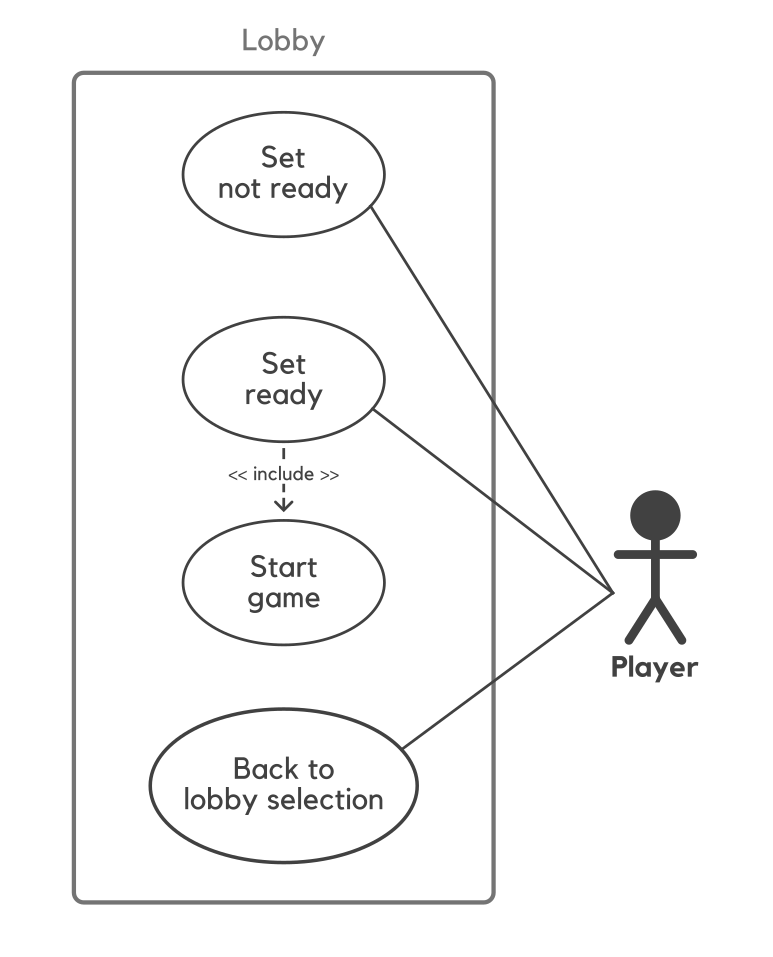
\includegraphics[width=0.5\textwidth]{figures/lobbyUseCase.png}}
      \hfill
      \subfloat[Match]{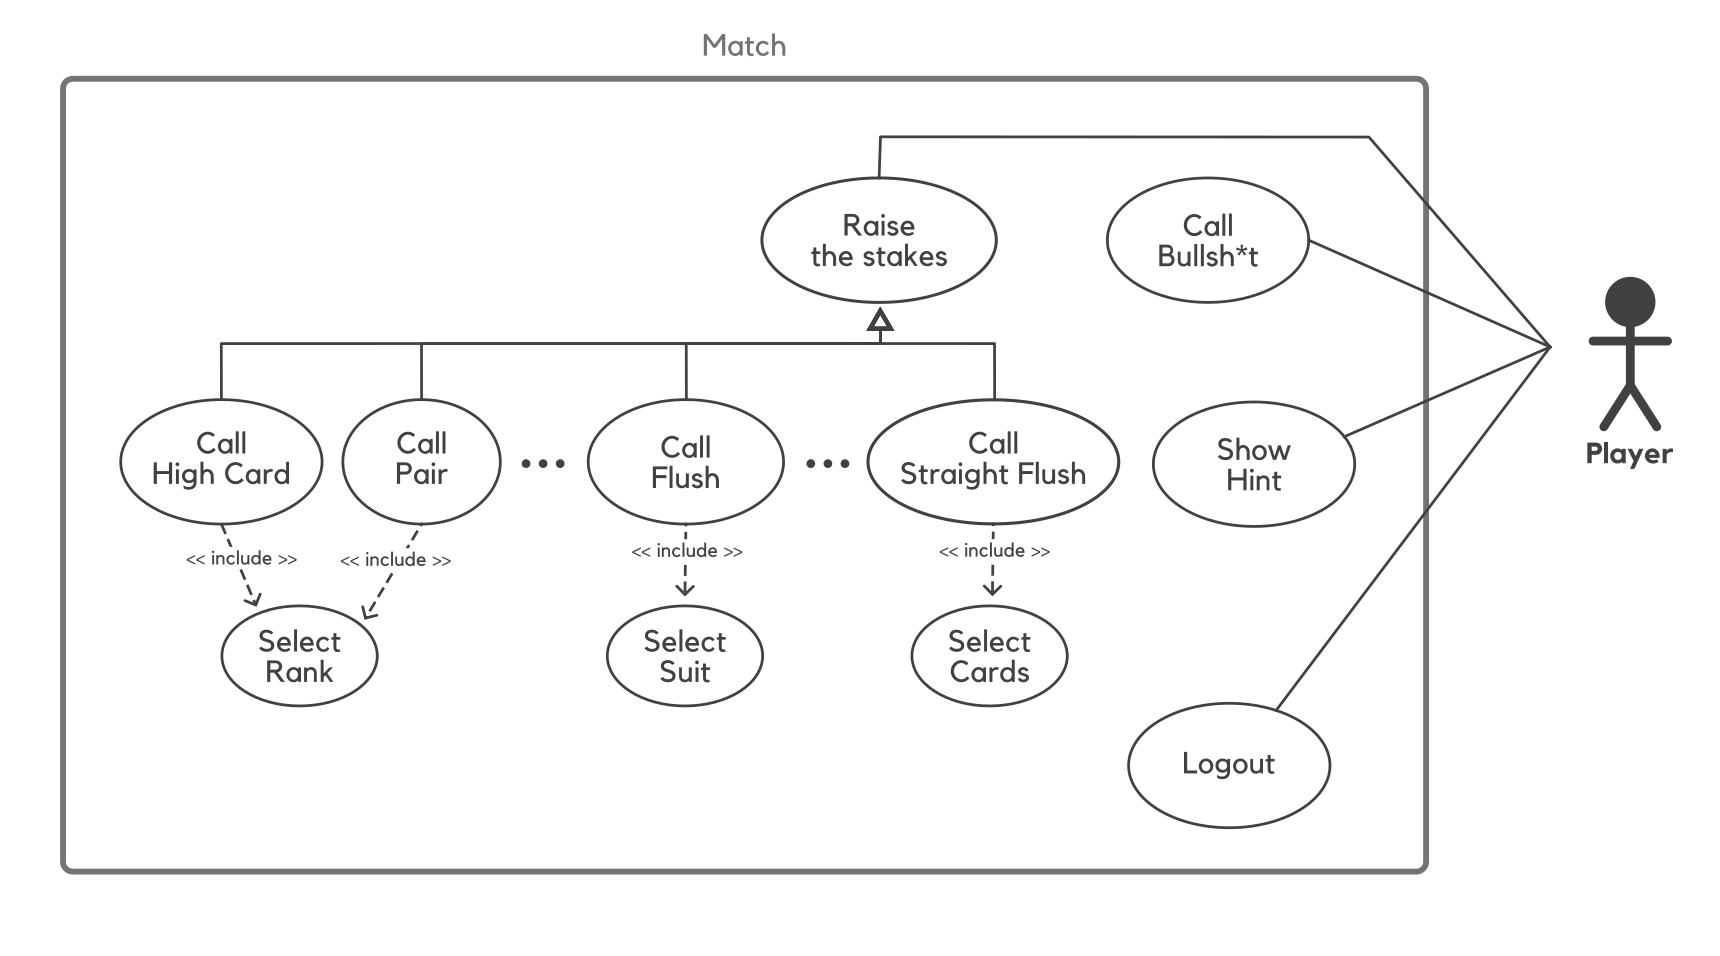
\includegraphics[width=1\textwidth]{figures/gameUseCase.png}}
      \caption{Use Case Diagrams}
      \label{fig:use-case-diagrams}
\end{figure}

\newpage
\section{Requirements}\label{requirements}
Starting from the concept, we can identify the following requirements for the application:

\subsection{Functional Requirements}\label{functional-requirements}
\begin{enumerate}
      \item \textbf{Lobby Creation}\par
            The application must allow users to create a new lobby and share the access code with
            friends.
      \item \textbf{Lobby Joining}\par
            The application must allow users to join a lobby by entering the access code.
      \item \textbf{Gameplay}\par
            The application must allow users to play Liar's Poker following the game rules.
\end{enumerate}

\subsection{Non-functional Requirements}\label{non-functional-requirements}
\begin{enumerate}
      \item \textbf{Scalability}\par
            The application must be able to handle multiple lobbies and games simultaneously.
            \begin{itemize}
                  \item \textbf{Acceptance Criteria:} The system must be able to handle at least 5
                        concurrent games.
            \end{itemize}
      \item \textbf{Fault Tolerance}\par
            The application must be able to handle user disconnections without losing a running game
            and should recover from server failures.
            \begin{itemize}
                  \item \textbf{Acceptance Criteria:} The system must be able to recover from server
                        failures within 1 minute.
            \end{itemize}
      \item \textbf{Consistency}\par
            The application must ensure that all players see the same game state at all times.
            \begin{itemize}
                  \item \textbf{Acceptance Criteria:} The system must ensure that all players see the
                        same game state within 2 second from the bullsh*t call.
            \end{itemize}
      \item \textbf{Performance}\par
            The application must be able to have good response times.
            \begin{itemize}
                  \item \textbf{Acceptance Criteria:} A new game must be created within 5 seconds.
            \end{itemize}
\end{enumerate}

\subsection{Glossary of cards combinations}\label{cards-combinations}
In this section we list all the possible cards combinations, that can be declared during the game,
ordered by increasing value:
\begin{enumerate}
      \item \textbf{High Card}\par
            In the combined cards of all players there is a card with the rank declared by the player.
      \item \textbf{Pair}\par
            In the combined cards of all players there are two cards with the same rank declared by
            the player.
      \item \textbf{Two Pair}\par
            In the combined cards of all players there are two pairs of cards with the same ranks
            declared by the player.
      \item \textbf{Three of a Kind}\par
            In the combined cards of all players there are three cards with the same rank declared by
            the player.
      \item \textbf{Straight}\par
            In the combined cards of all players there are five cards with consecutive values declared
            by the player.
      \item \textbf{Flush}\par
            In the combined cards of all players there are five cards with the same suit declared by
            the player.
      \item \textbf{Full House}\par
            In the combined cards of all players there is a \emph{pair} and a \emph{three of a kind}
            with the respective ranks declared by the player.
      \item \textbf{Four of a Kind}\par
            In the combined cards of all players there are four cards with the same value declared
            by the player.
      \item \textbf{Straight Flush}\par
            In the combined cards of all players there are five cards with consecutive values and
            the same suit declared by the player.
      \item \textbf{Royal Flush}\par
            In the combined cards of all players there are five cards with the same suit declared
            by the player and the ranks \emph{10}, \emph{J}, \emph{Q}, \emph{K} and \emph{Ace}.
\end{enumerate}

\newpage
\section{Design}\label{design}
\subsection{Architecture}\label{architecture}
The architecture of the system follows the standard MVC principle:
\begin{itemize}
      \item Model are the classes that represent players and cards
      \item View is UI realized with Web components
      \item Controller is the class that manages the game logic
\end{itemize}
For the communication architecture and the distributed part, we opted for a client-server architecture
using a publish-subscribe pattern.

The idea is that the broker manages the communication between the clients and the server, and the
server manages the game logic.

When requested by a player, the server creates a new lobby where other players can join. Every time
a new player joins the lobby, it automatically subscribes to the game topics.

All the clients are subscribed to the same topic, so they can receive the messages from the server
(e.g. moves, game status, etc.).

We choose this architecture because it is simple and suitable for our project.
In fact, using a publish-subscribe architecture, clients don't have to request the server for the game
status, but they receive it automatically when the server publishes it
(and so on for the other messages).

\subsection{Infrastructure}\label{infrastructure}
\begin{itemize}
      \item Both players and server are components of the pub-sub model.
      \item There is one server that manages the game logic.
      \item There is a broker that manages the communication between the clients and the server.
      \item Data aren't store permanently, so there is no need for a database.
      \item There aren't authentication mechanisms so every one who knows the broker address can join
            the game.
\end{itemize}
Components are distributed over all the network, so they can be on different machines and different
networks. For simplicity, we used the same network for all the components and the same machine both
for server and broker.

To find each other, the components use the broker address and the topics to which they have to
subscribe or publish; so clients are only required to know the broker address to join the game.

Components are named using a nickname that everybody choose on game launch.

The pub-sub behaviour is shown in \cref{fig:pubsubdiagram}. Dotted lines are for subscribe messages,
while solid lines are for publish messages.

\begin{figure}
      \centering
      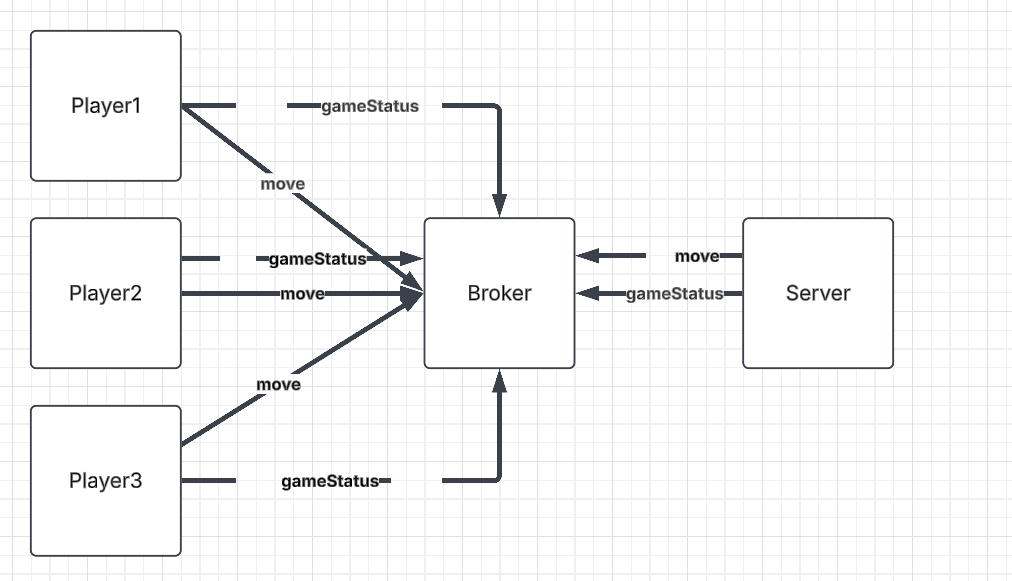
\includegraphics[width=0.5\textwidth]{figures/pubsubdiagram.png}
      \caption{Architecture diagram}
      \label{fig:pubsubdiagram}
\end{figure}

\subsection{Modelling}\label{modelling}
The system will be fundamentally composed by the classes shown in \cref{fig:classes}.

Each component models the real world entities that are needed to play the game in a non-distributed
way.
\begin{figure}
      \centering
      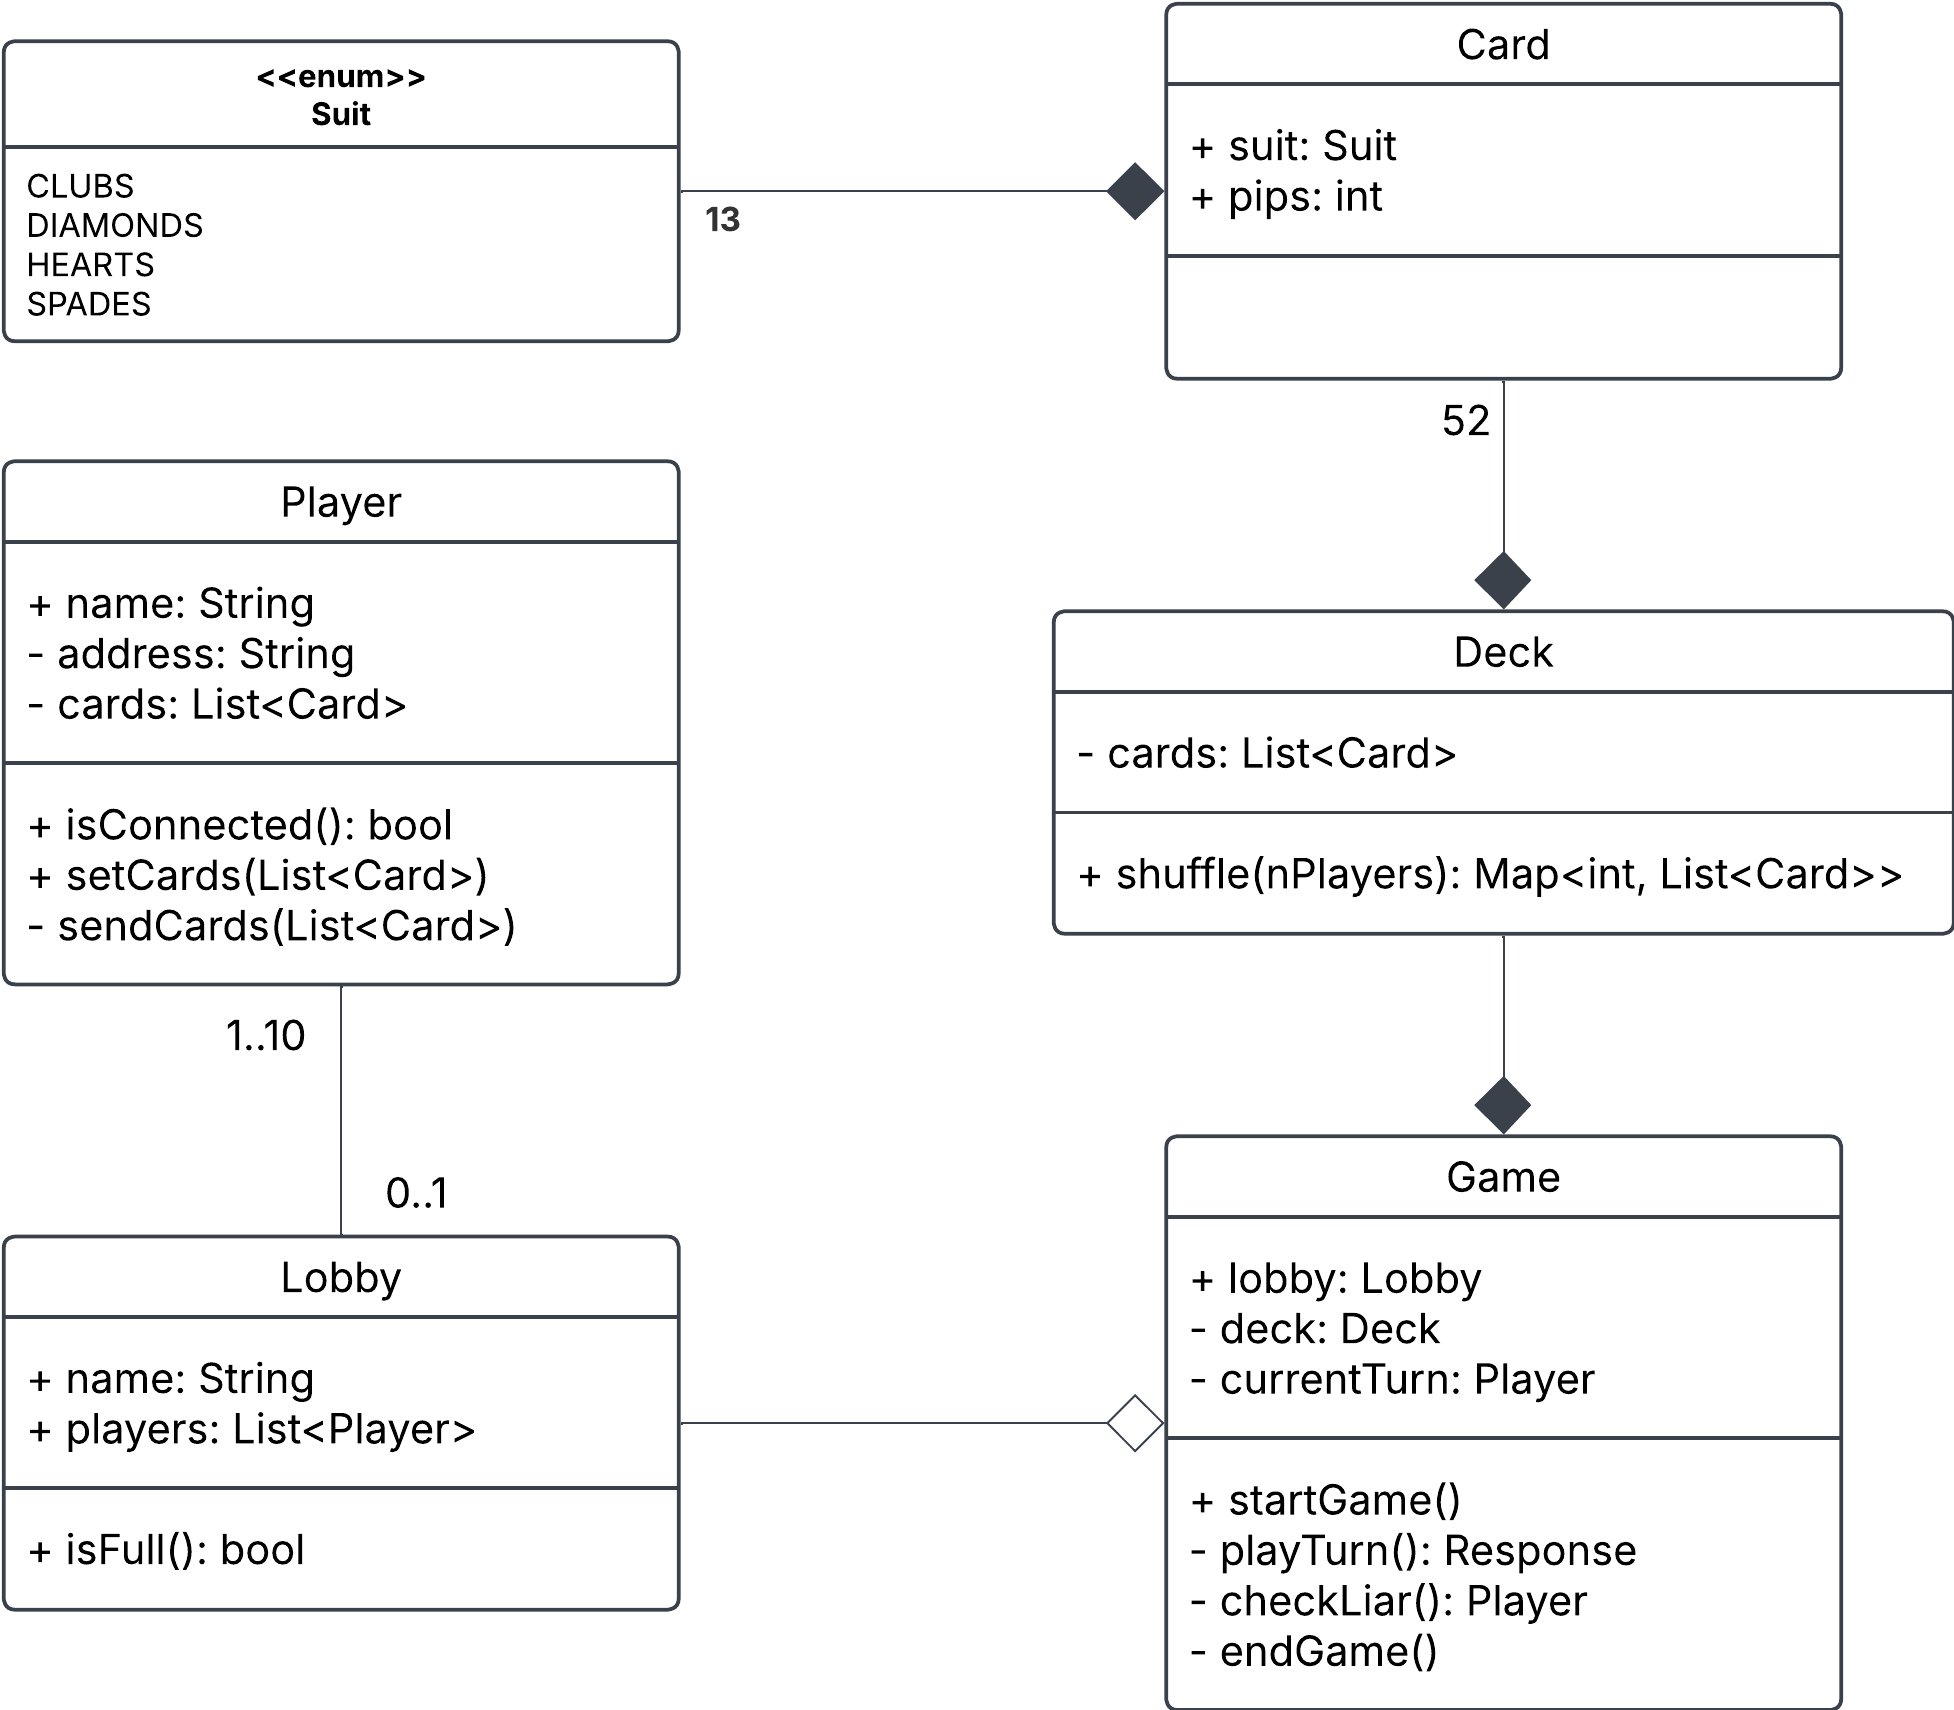
\includegraphics[width=0.8\textwidth]{figures/classes.png}
      \caption{Class diagram of the system}
      \label{fig:classes}
\end{figure}

The game is the most important entity of the whole model. It has a deck of cards, that can be shuffled,
and a set of players, each one with: a nickname, its given cards and its lobby ready state.
To handle the game logic it keeps in memory the current player and the latest raise.

It can be asked to:
\begin{itemize}
      \item Add or remove a player from the game
      \item Get a fresh set of shuffled cards for the players
      \item Raise the stakes and advance the turn with the new minimum stake
      \item Check if the latest stake was a lie
      \item Get the currently playing user
      \item Get the player that raised the stakes
\end{itemize}

At the core of the entire system are messages, these, given the simple nature of the game,
are quite simple too: containing a single object that represents the move the player wants to make or
the response of the server.

The real difference and context of the message is given by the topic to which it is published.

All the topics used by the system can be viewed in it's associated enum but are not directly
used when sending a message since most of them are different depending on the context in which they are used.
For example the "remove player" topic is used as it is when logging out a player that is not
in a game, but when used in a game it will be linked together with the lobby ID.
Most notably these are the topics used when playing:
\begin{itemize}
      \item \textbf{Start Turn} \par
            The game publishes the current player and the minimum stake for him.
      \item \textbf{Start Round} \par
            The game publishes the list of all players and their cards at the start of a round.
      \item \textbf{Round Loser} \par
            The game publishes the player that lost the round and all the cards in game,
            also indicating if the player was eliminated.
      \item \textbf{Raise Stake} \par
            The player informs the game of his new stake.
      \item \textbf{Check Liar} \par
            The player doubts the previous stake and asks the game to check if it was a lie.
      \item \textbf{Game Over} \par
            The game publishes the winner signalling the end of the game.
      \item \textbf{Remove Player} \par
            The player announces that he will log out of the game.
      \item \textbf{Game Info} \par
            If a player tries to reconnect to a game, the game will publish the current game state
\end{itemize}

\subsection{Interaction}\label{interaction}
Components communicate over the network using the MQTT protocol so using a Message Broker pattern.
Using this pattern, publishers can send messages without knowing who is going to receive them, and
subscribers can receive messages without knowing who sent them.
The broker is the one who manages the communication between the clients and the server, so the clients
don't have to know the server address, but only the broker address; moreover, the server has
to know the broker address to publish messages, but it doesn't have to know the clients' addresses.

This kind of architecture is highly decoupled, so the components can be easily replaced or modified
without affecting the others.

The following list will explain the interaction between the components in more detail.

\begin{itemize}
      \item \textbf{Connection} \par
            The connection behaviour is shown and explained in \cref{fig:connection}.
            \begin{figure}
                  \centering
                  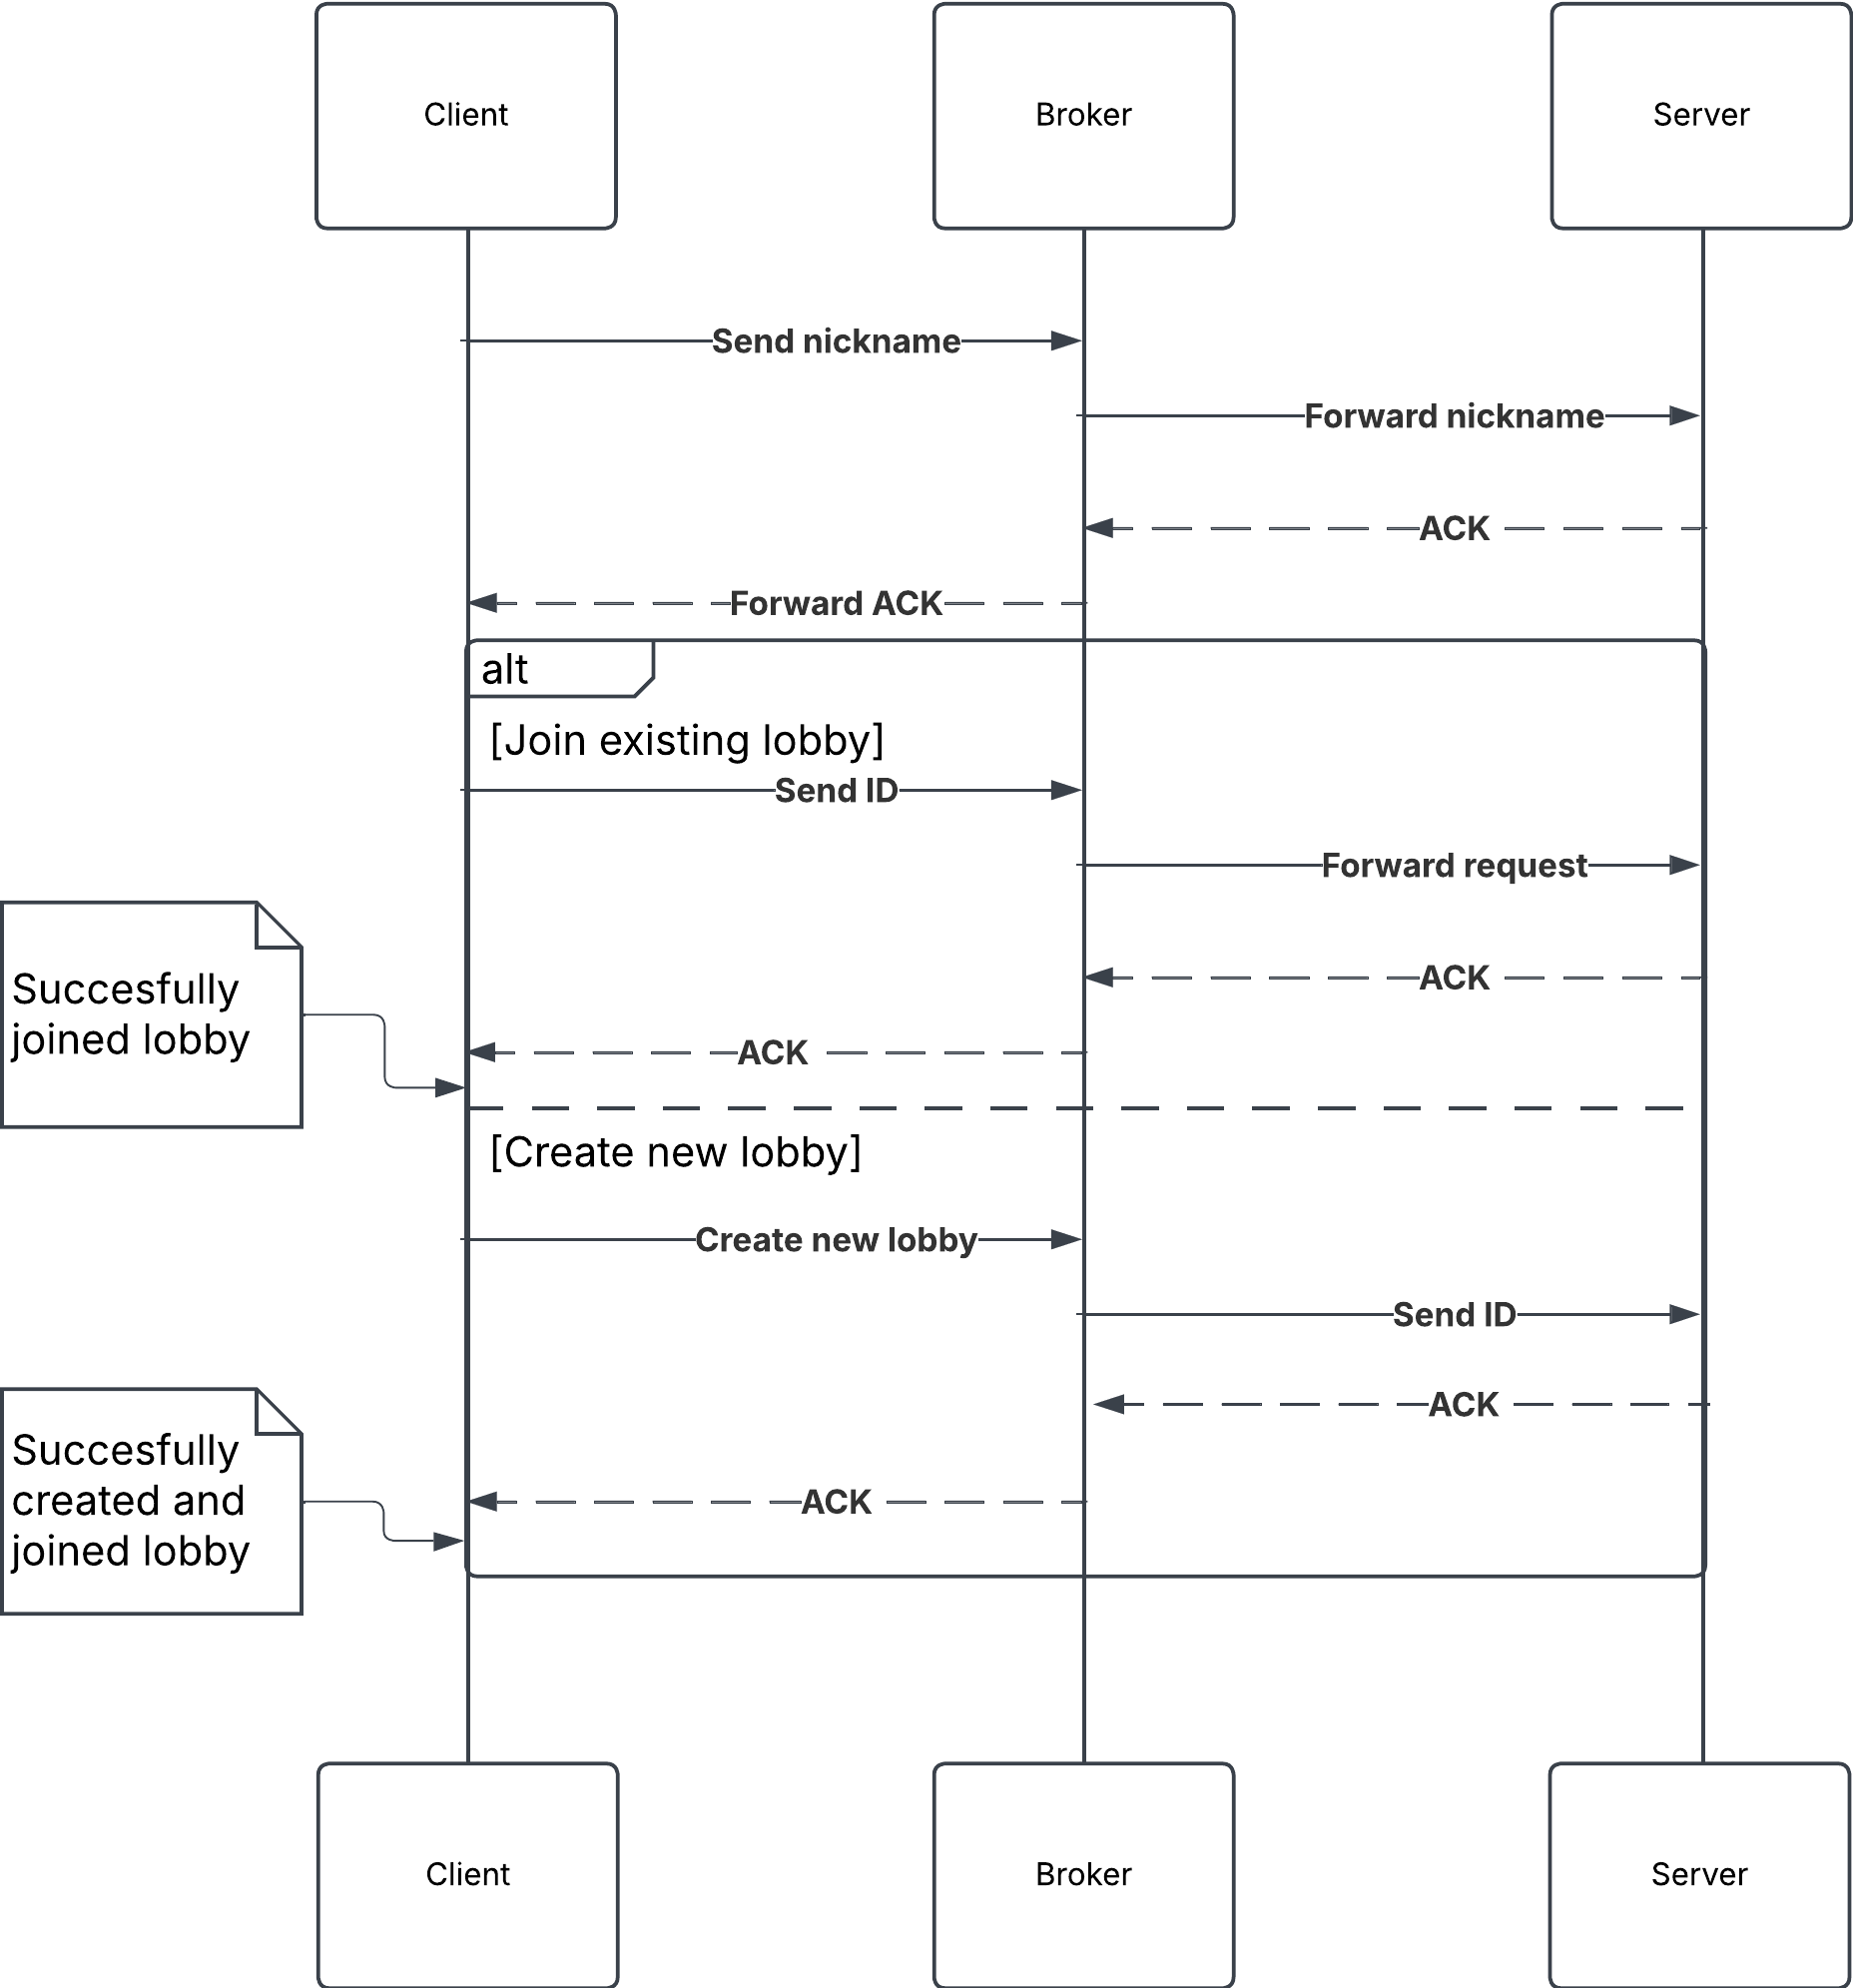
\includegraphics[width=0.8\textwidth]{figures/sequenceConnection.png}
                  \caption{Sequence diagram of the connection phase}
                  \label{fig:connection}
            \end{figure}
      \item \textbf{Game Move} \par
            The game move behaviour is shown and explained in \cref{fig:game-move}.
            \begin{figure}
                  \centering
                  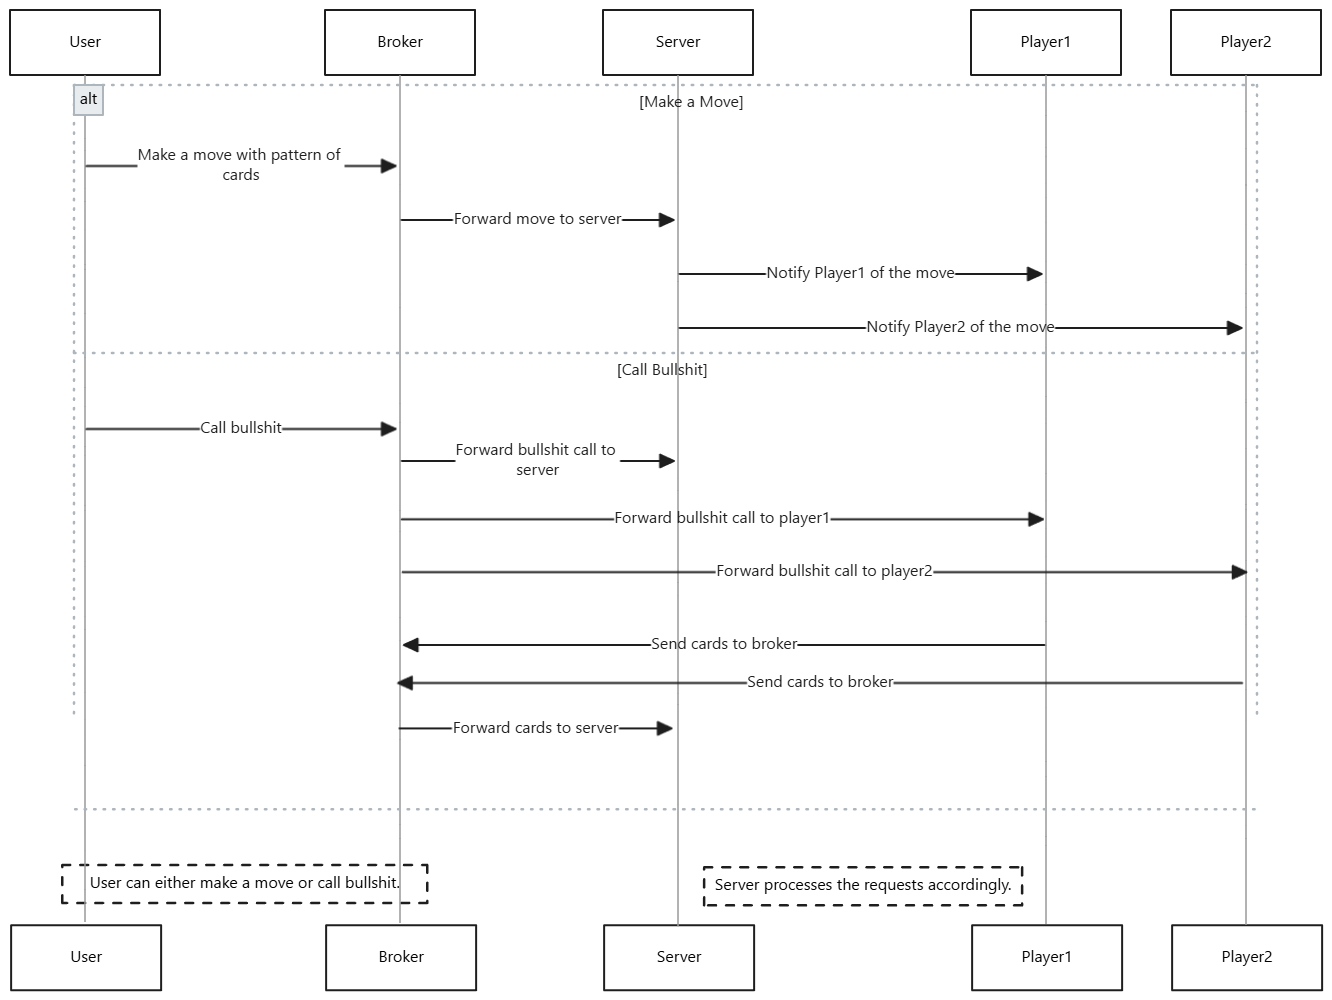
\includegraphics[width=0.8\textwidth]{figures/sequenceGameMove.png}
                  \caption{Sequence diagram of a generic game move}
                  \label{fig:game-move}
            \end{figure}
      \item \textbf{End Game} \par
            The end game behaviour is shown and explained in \cref{fig:end-game}.
            \begin{figure}
                  \centering
                  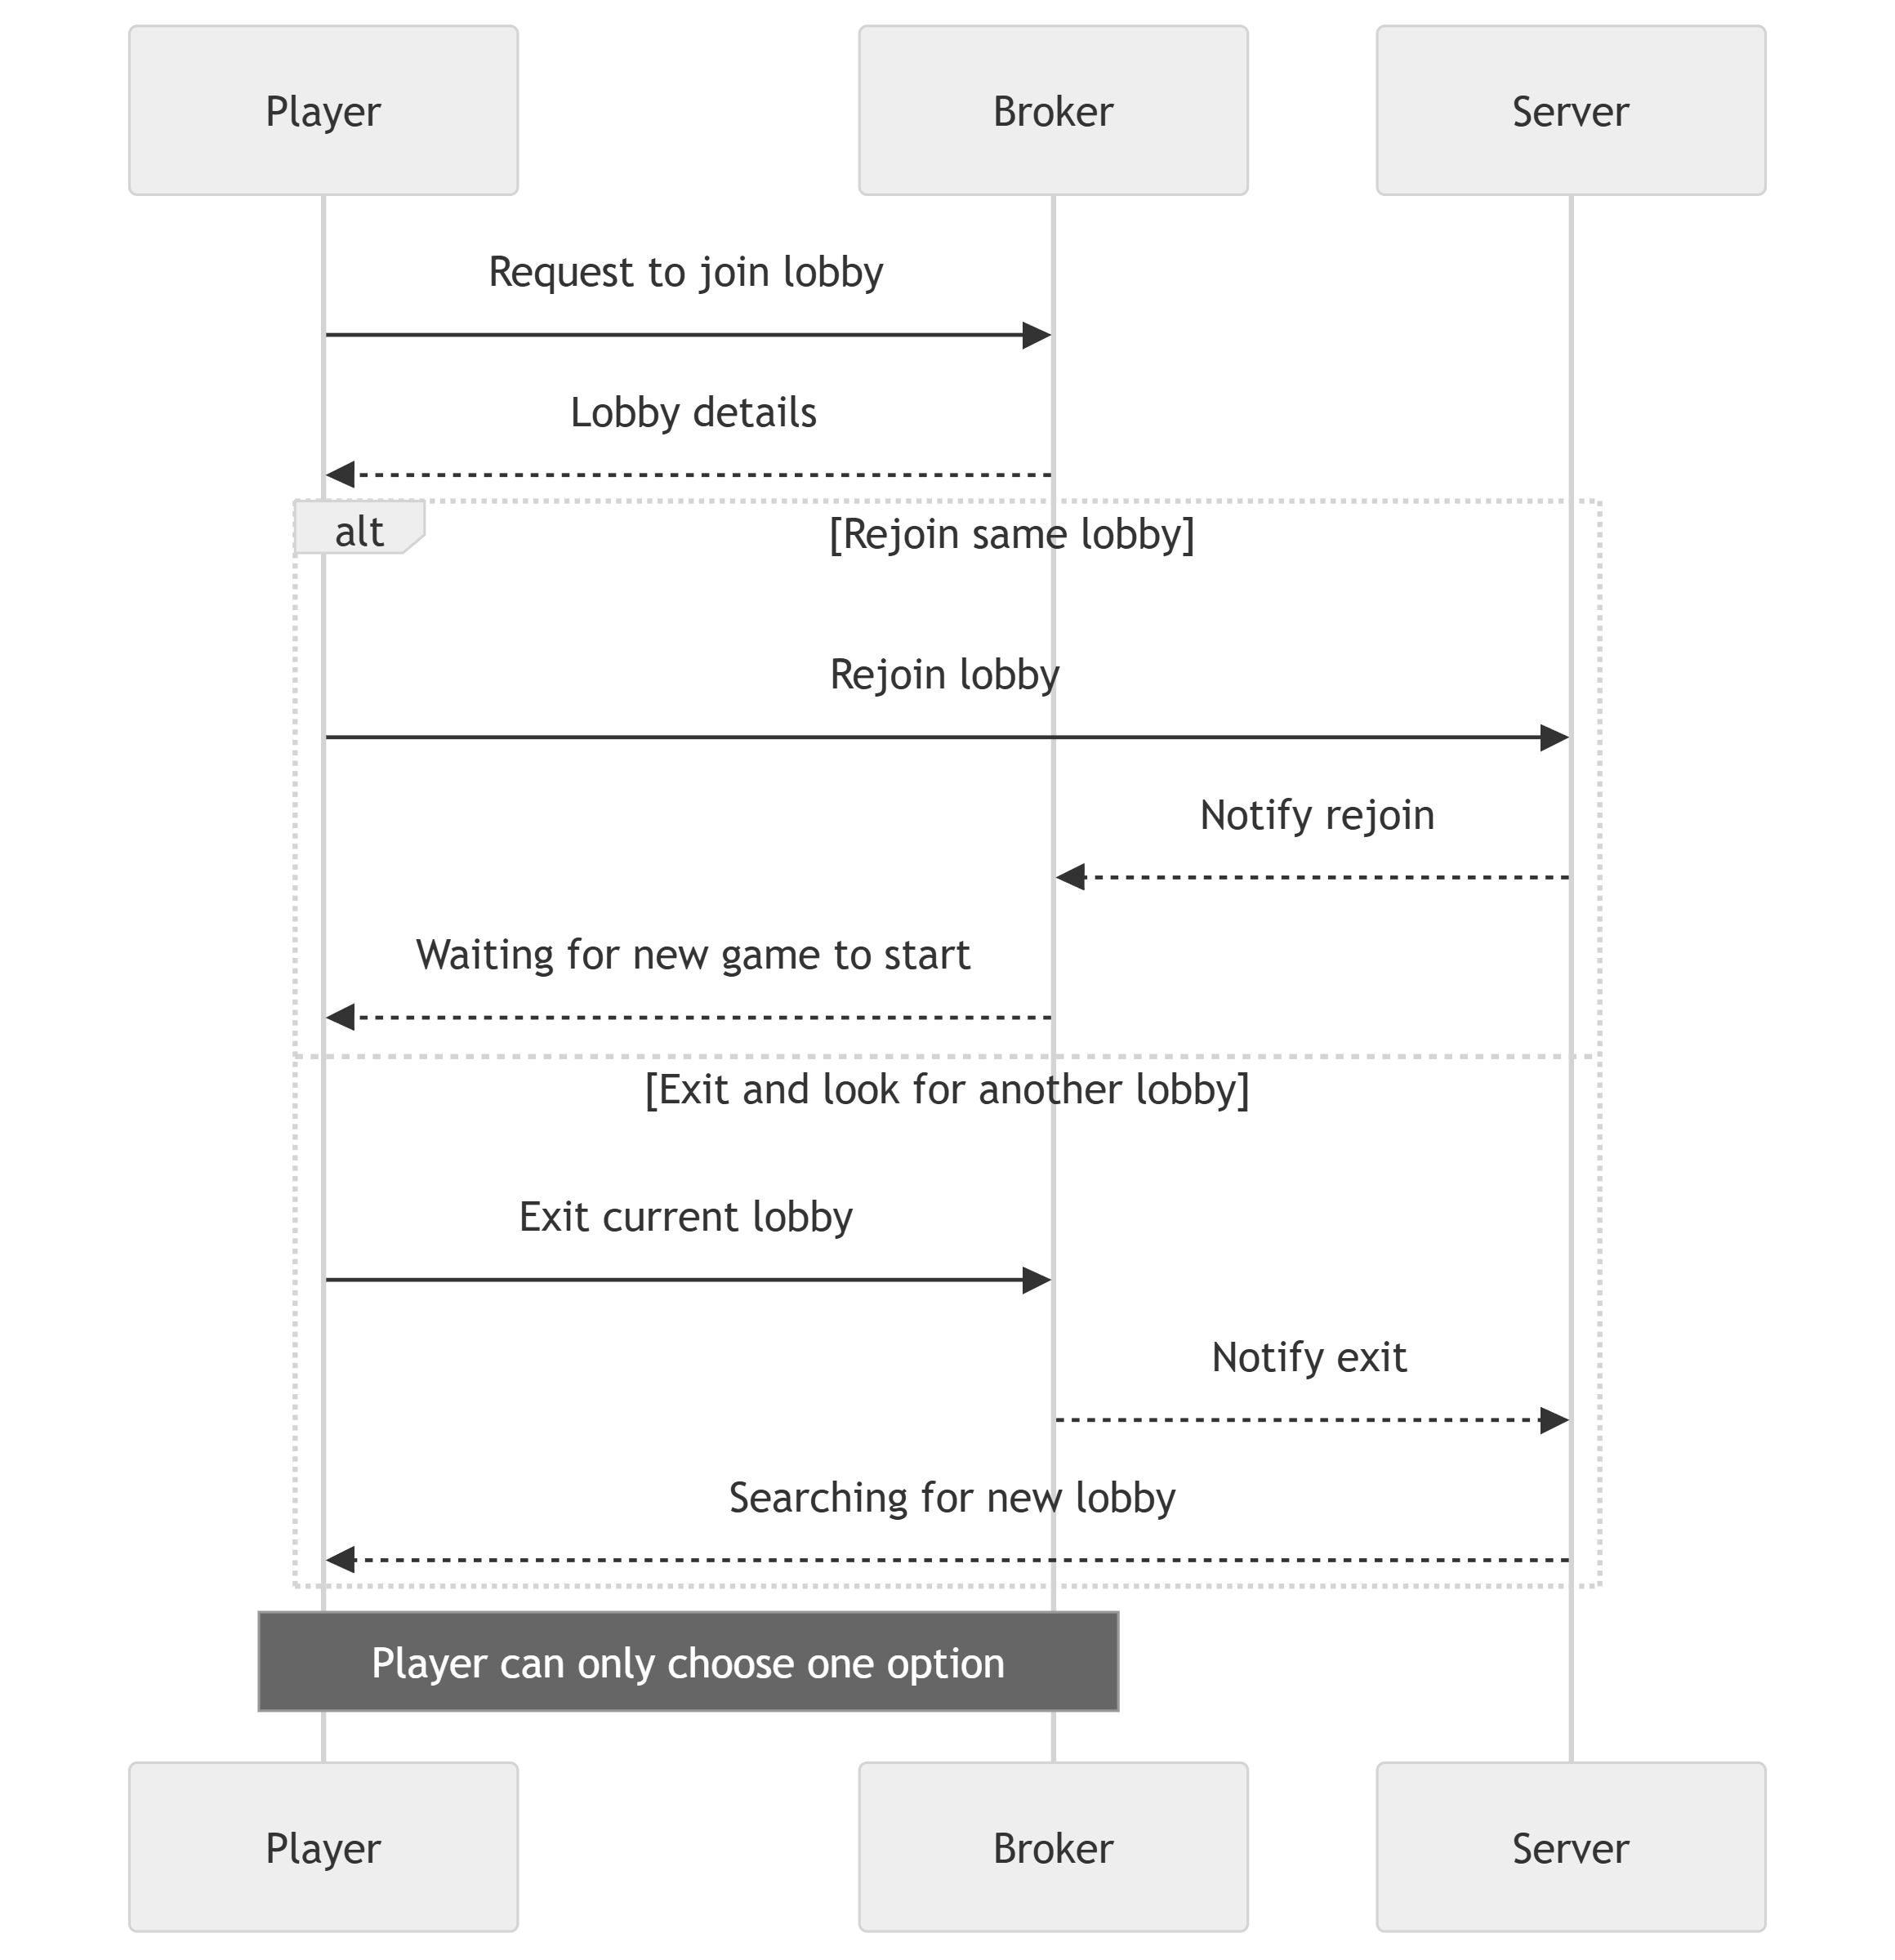
\includegraphics[width=0.8\textwidth]{figures/sequenceEndGame.png}
                  \caption{Sequence diagram of end game phase}
                  \label{fig:end-game}
            \end{figure}
\end{itemize}
\newpage
\subsection{Behaviour}\label{behaviour}
Many actors are needed to keep the game going and to manage the communication between them.

The following are all the components actually needed and their behaviours:
\begin{itemize}
      \item
            \textbf{The client} \cref{fig:clientStates} \par
            The client starts by establishing a connection to the MQTT broker, since it's fundamental
            for each part of the system.

            Right after it asks the player for their name and waits for the server approval.
            If the request is successful, the client can now choose to join or create a lobby.

            A player can set its status to ready when waiting for a game to start. Only when everyone
            is ready the server will send a message to start the game.

            When the game starts, the client waits for the server to publish the game status to
            show the interface to the player.
            The client can only send messages to the server when it is his turn, either rising the
            stakes or calling bullsh*t. If a player loses the match then he can only wait for it to
            finish. The player leaves the lobby only when a winner is found. When the game ends the
            player is put back into the same lobby and can either wait for a new game to start or look
            for a new one.

            At any point during the process the player can leave or be disconnected.
            If the player attempts to reconnect during a game the system will try to resume the status
            of the match.
            \begin{figure}
                  \centering
                  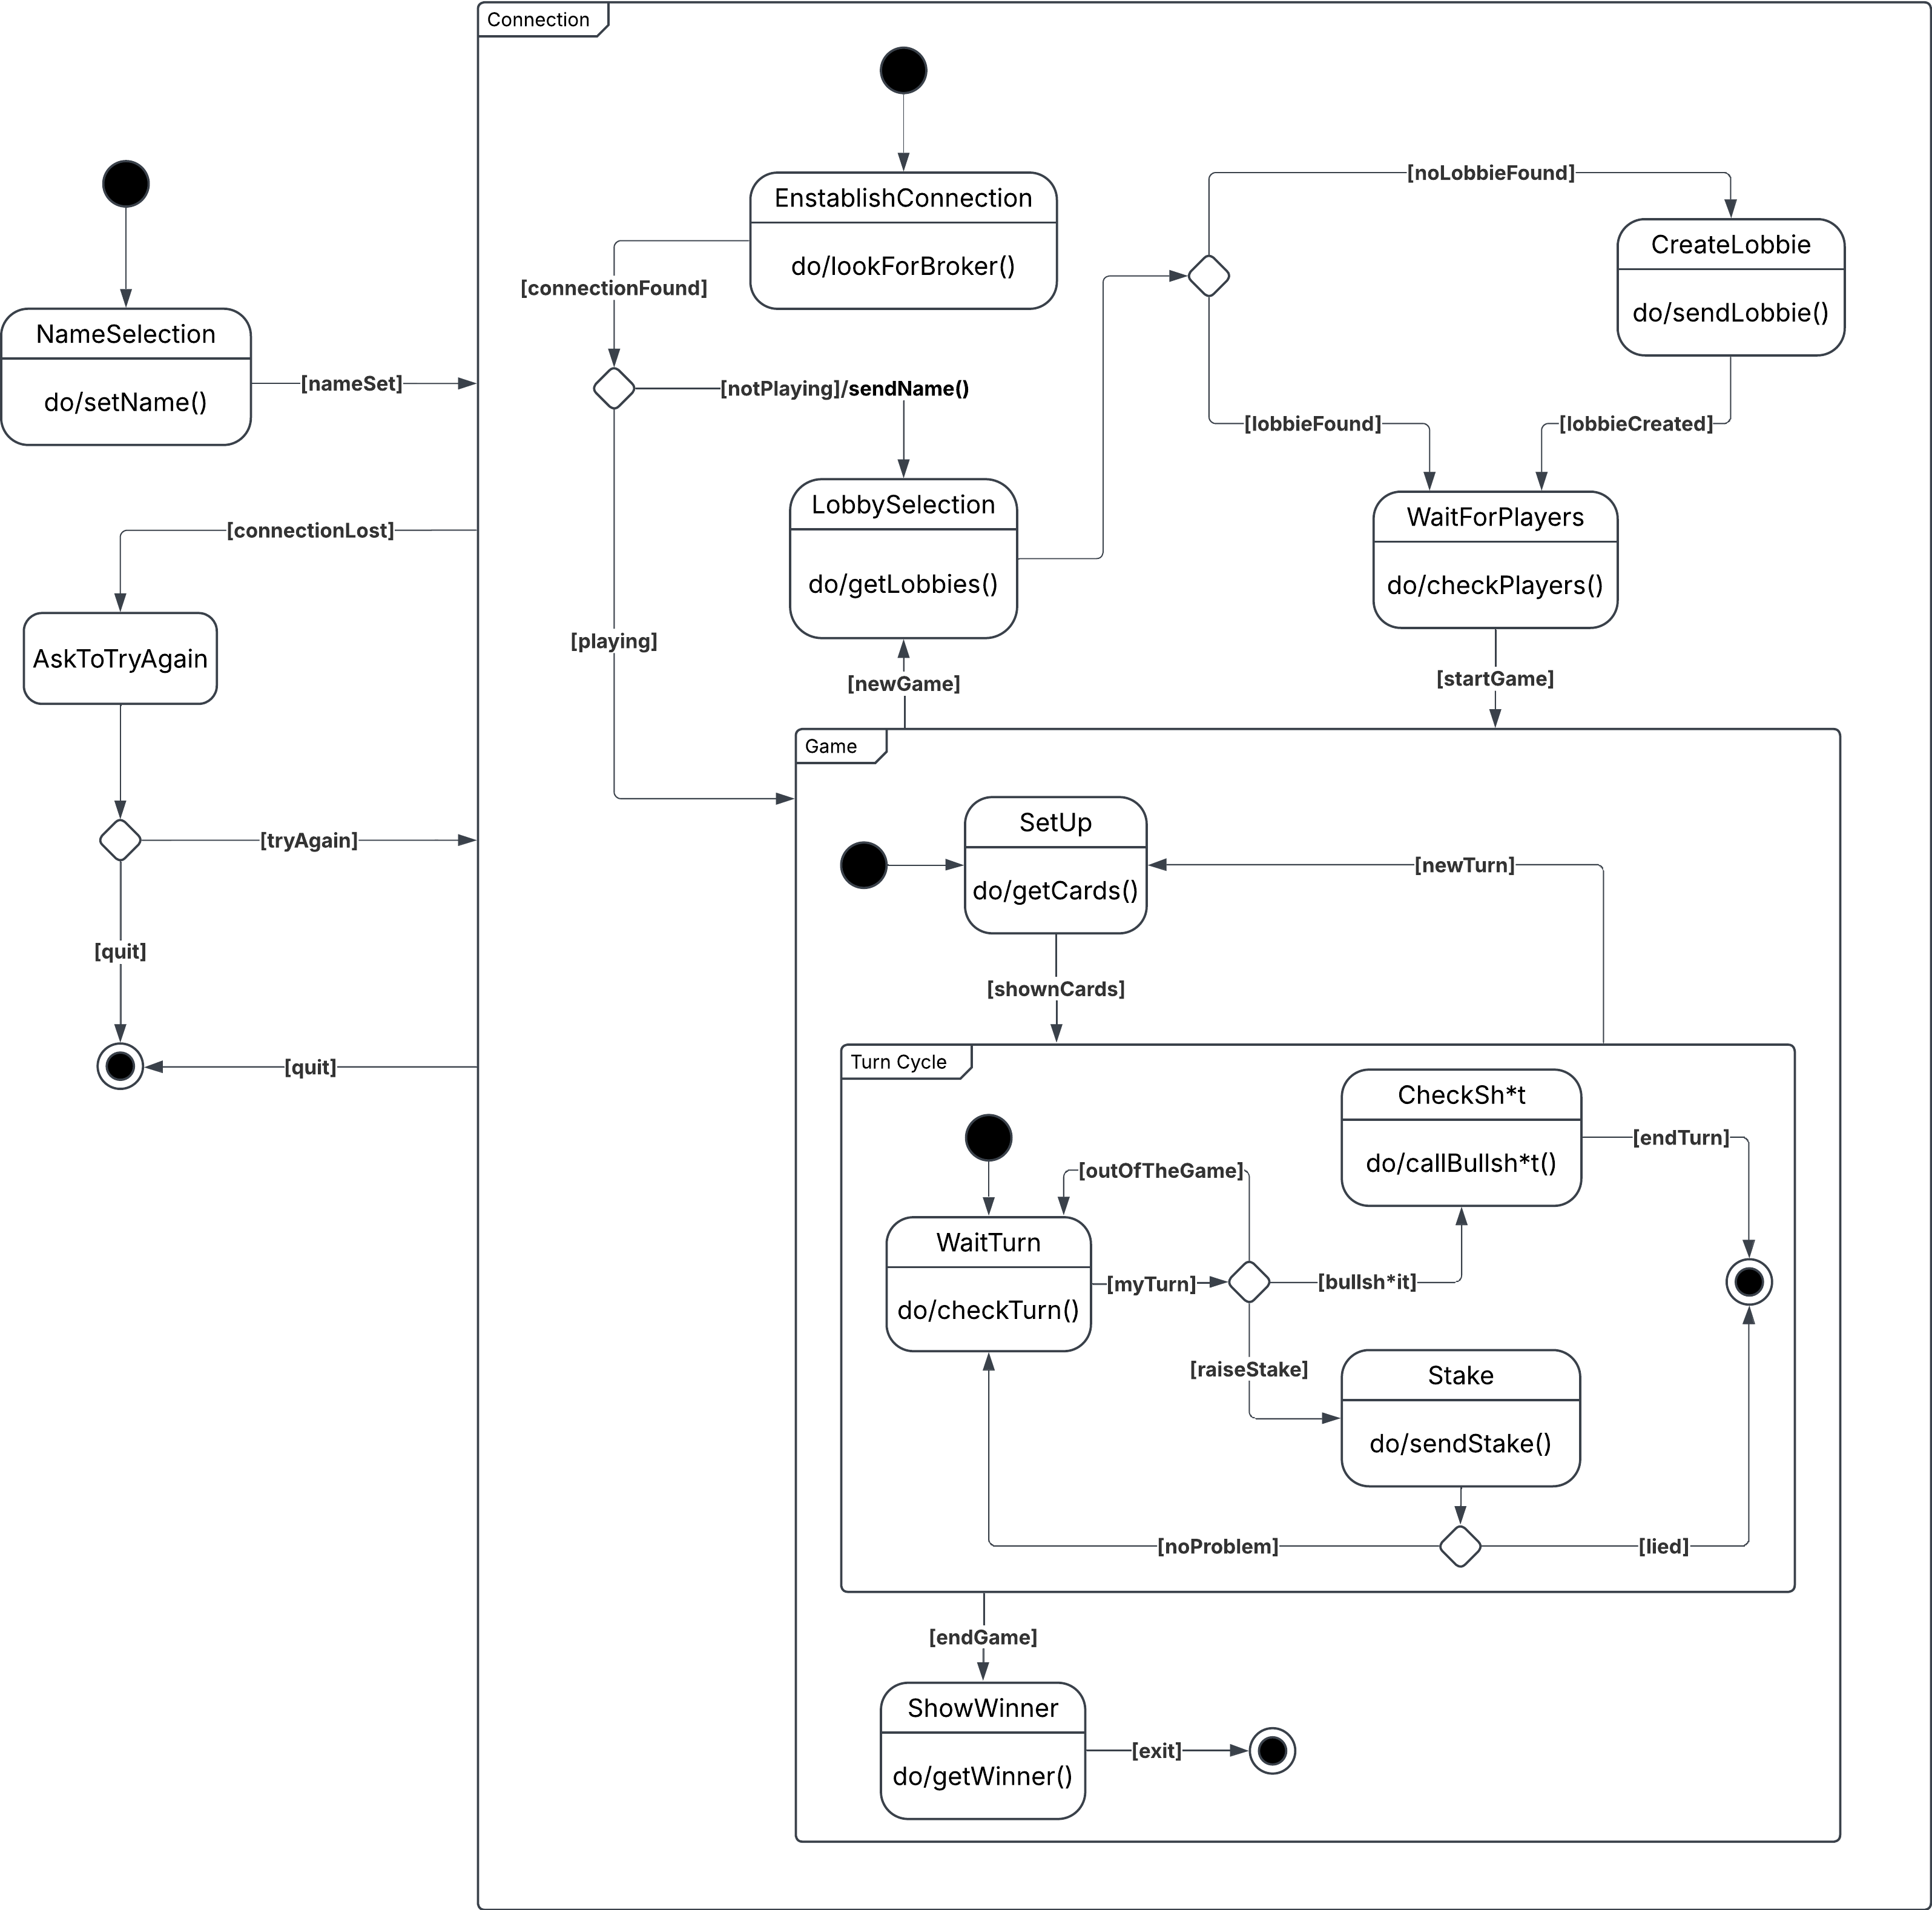
\includegraphics[width=0.8\textwidth]{figures/clientStates.png}
                  \caption{State diagram of the client}
                  \label{fig:clientStates}
            \end{figure}
      \item
            \textbf{The server} \cref{fig:serverStates} \par
            The server is mainly in charge of connecting new players and creating lobbies,
            delegating the game logic to different agents.

            At any point in time a new player can ask to connect or disconnect himself, causing the
            need to check whether the player was alone in a lobby, deleting it if left empty.
            The players connected can also ask to create or join a new lobby and, when everyone is ready,
            it will launch a new game instance.
            \begin{figure}
                  \centering
                  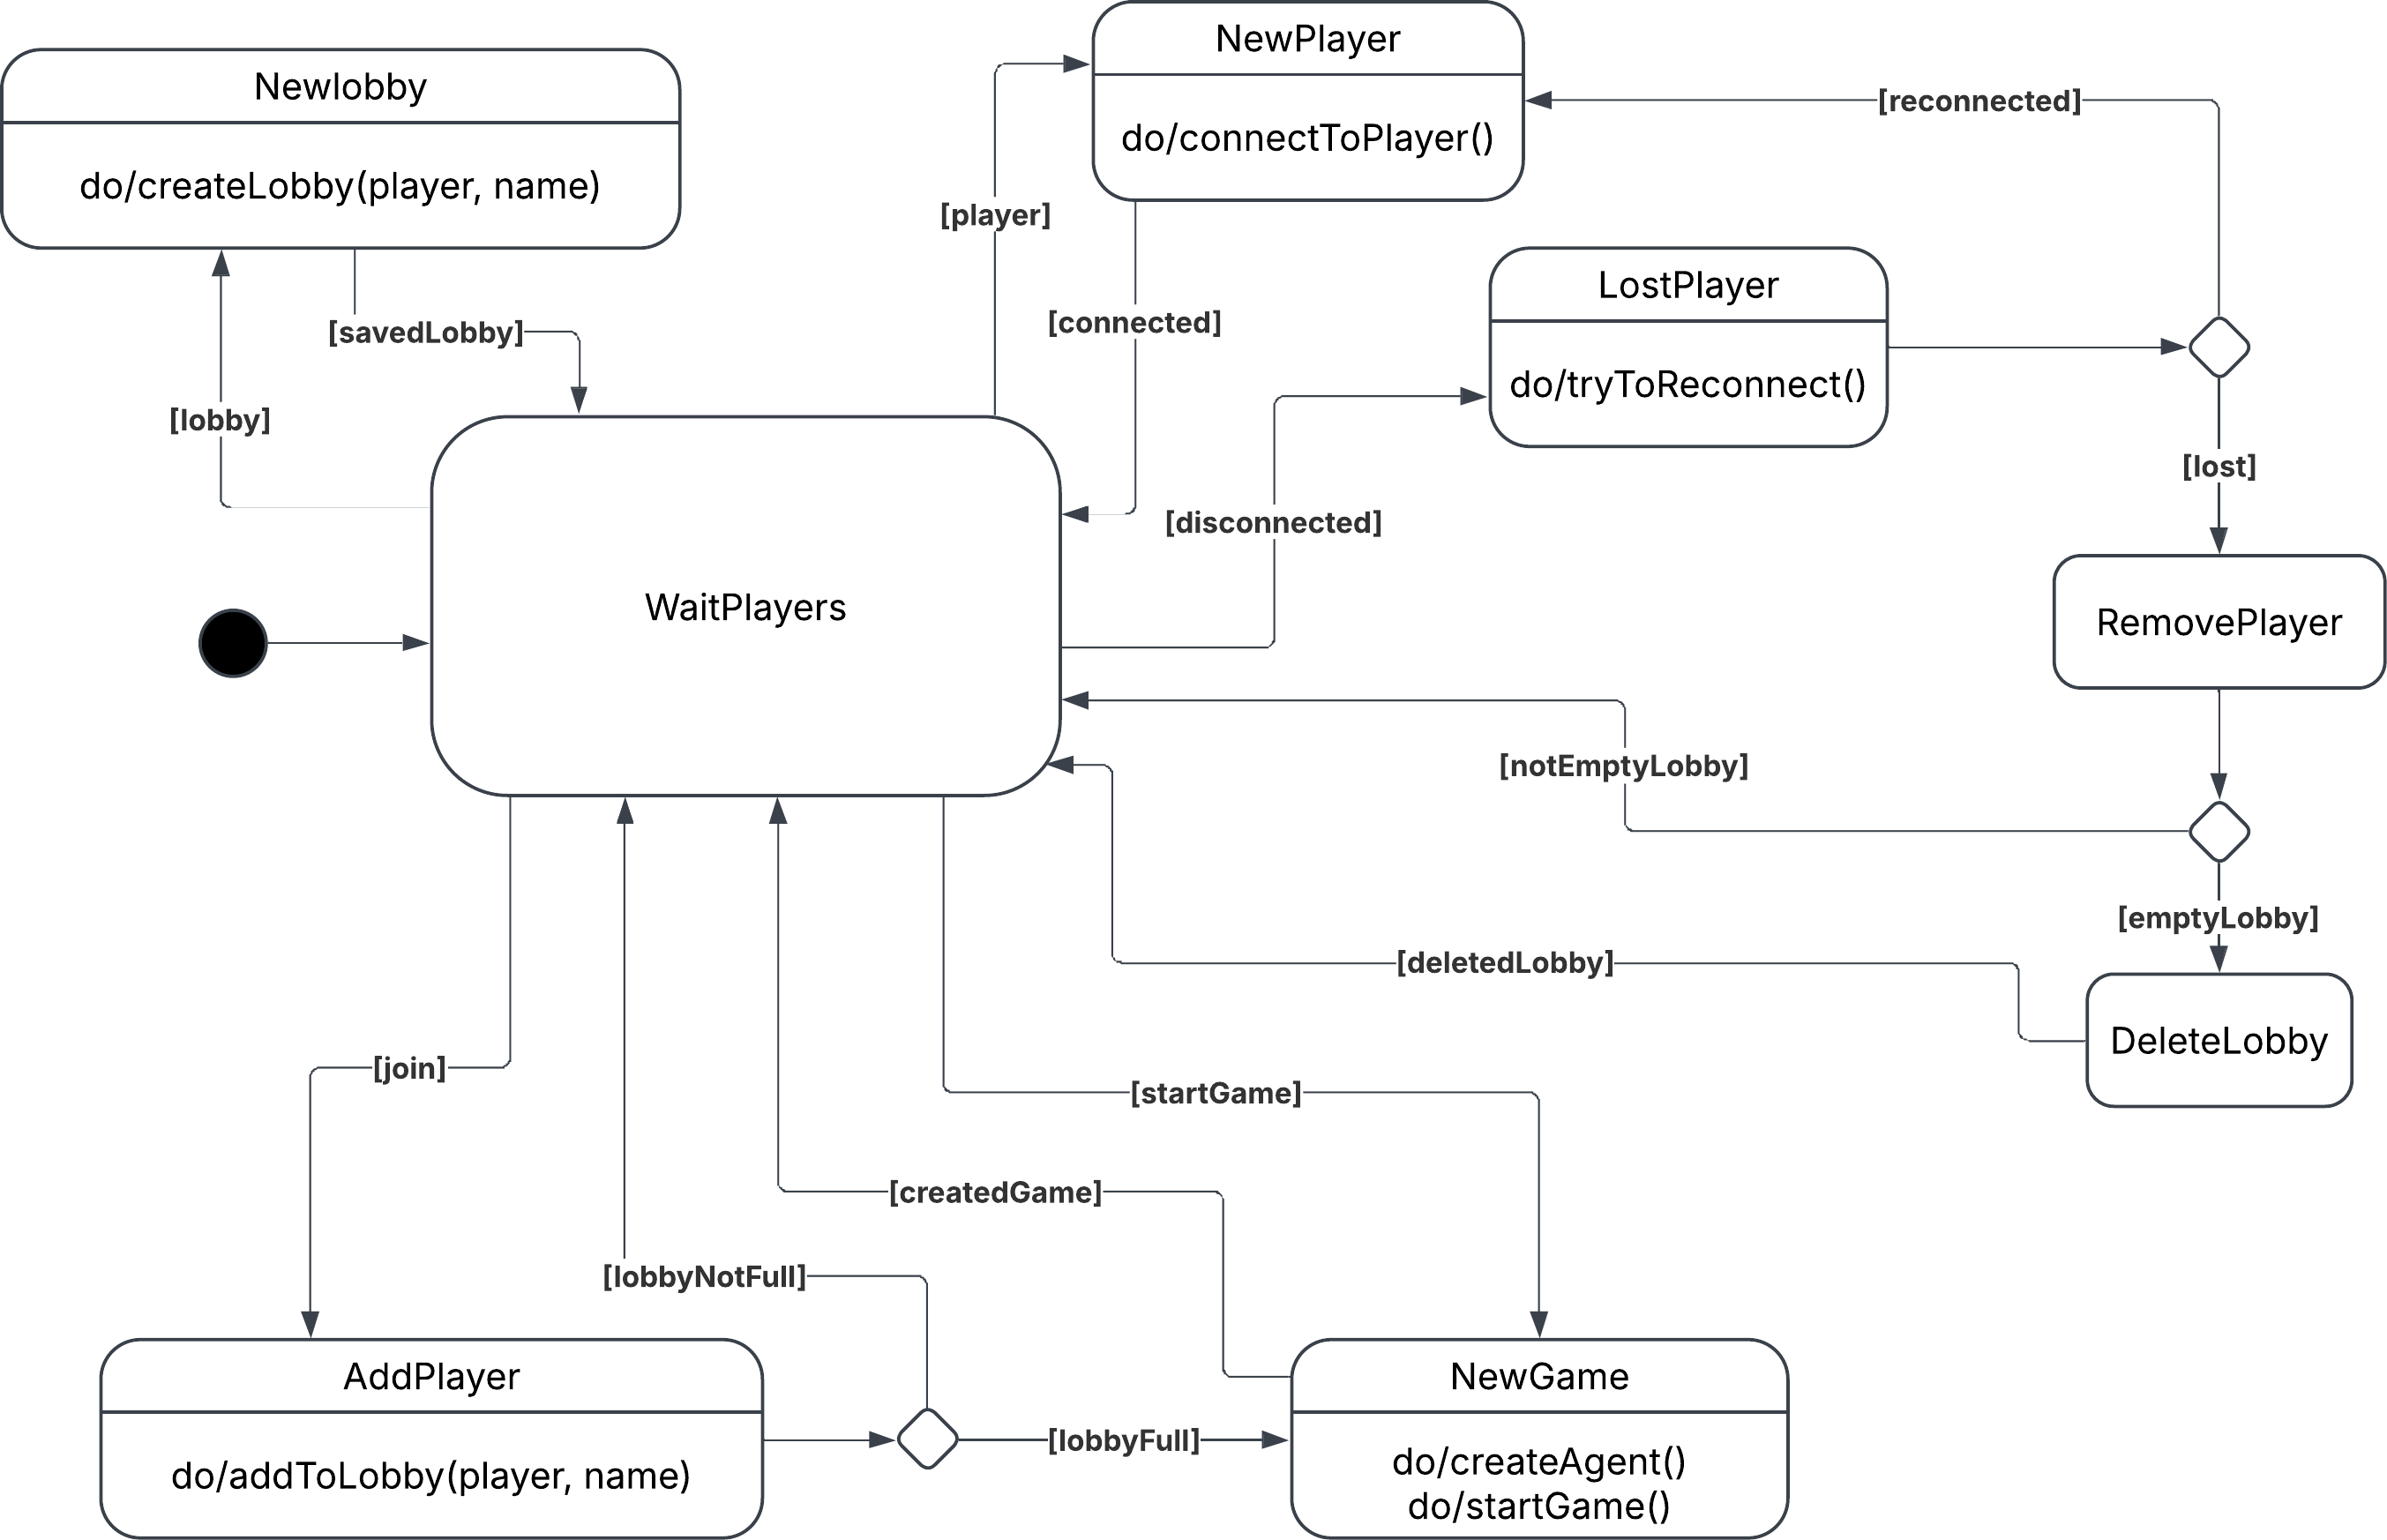
\includegraphics[width=0.8\textwidth]{figures/serverStates.png}
                  \caption{State diagram of the server}
                  \label{fig:serverStates}
            \end{figure}
      \item
            \textbf{The broker} \cref{fig:brokerStates} \par
            The broker is the central core to all communications between all the components.
            Always active using the MQTT standard.
            \begin{figure}
                  \centering
                  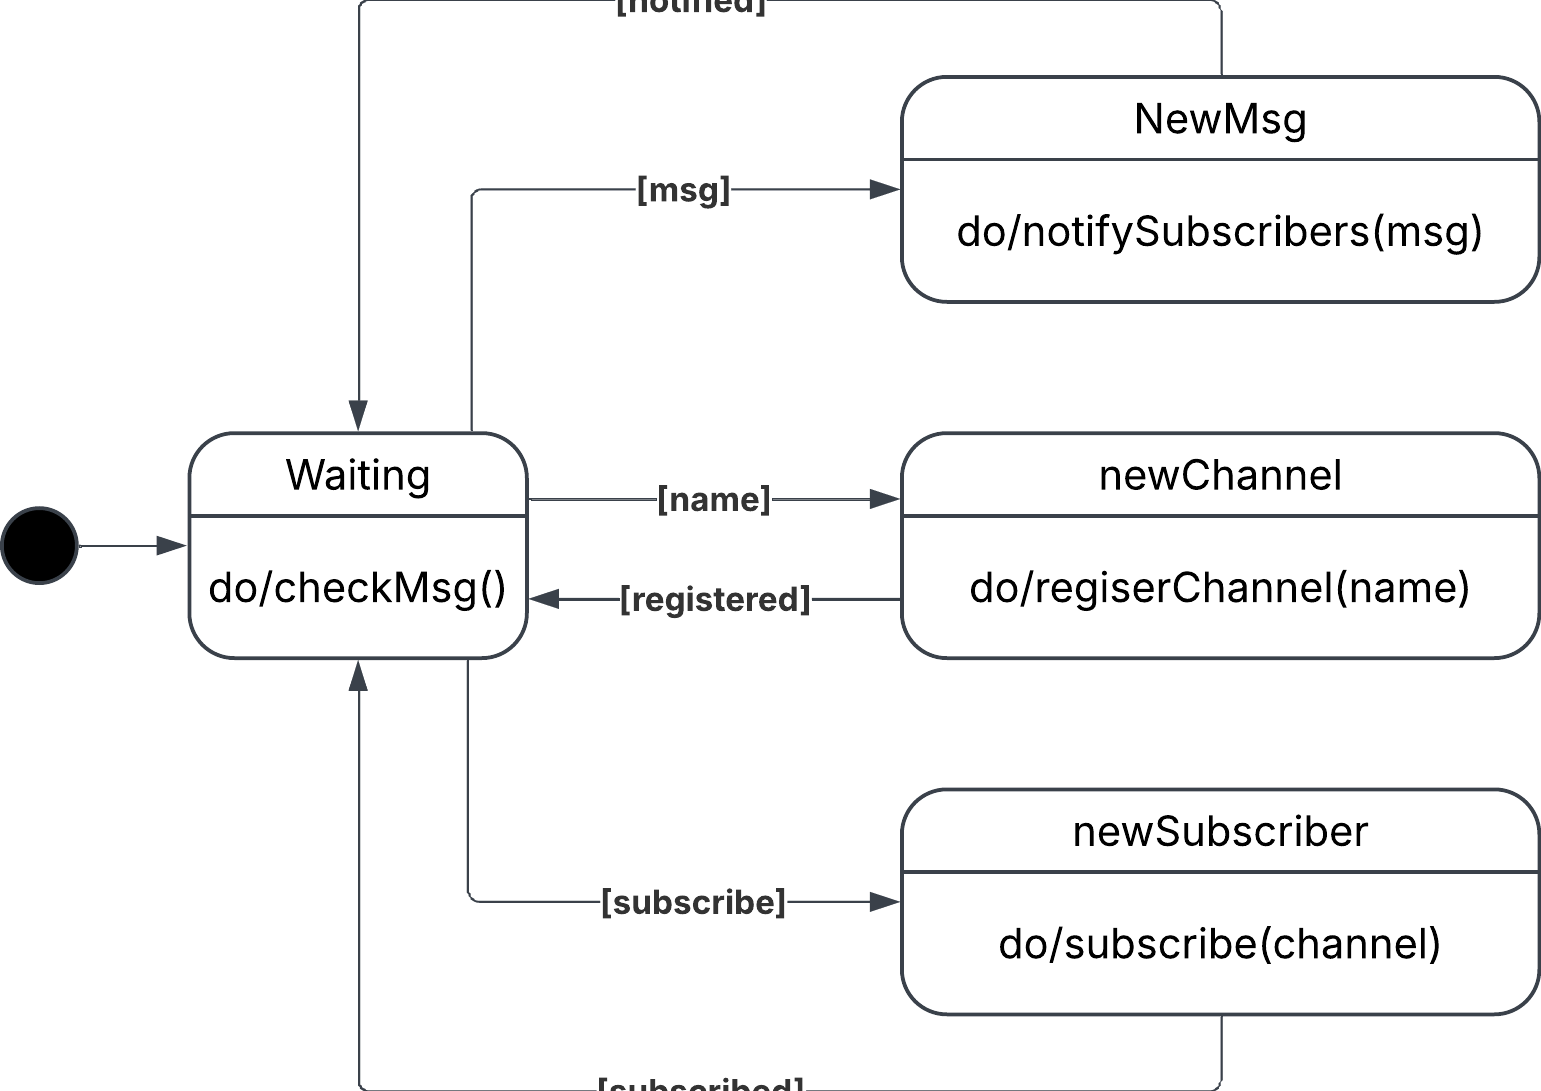
\includegraphics[width=0.8\textwidth]{figures/brokerStates.png}
                  \caption{State diagram of the broker}
                  \label{fig:brokerStates}
            \end{figure}
      \item
            \textbf{The game agent} \cref{fig:gameAgentStates} \par
            The game agent is a part of the server that takes on the role of managing the single
            matches. It is in charge of managing the game state, the players' moves and the game logic.

            Every time a player rises the stake, it calculates and sends the next minimum stake that
            the next player can make.
            It only waits for a minute for each player to make a move, if the player does not make a
            move in time, the game agent will kick him from the game and the game will continue with
            the remaining players.
            \begin{figure}
                  \centering
                  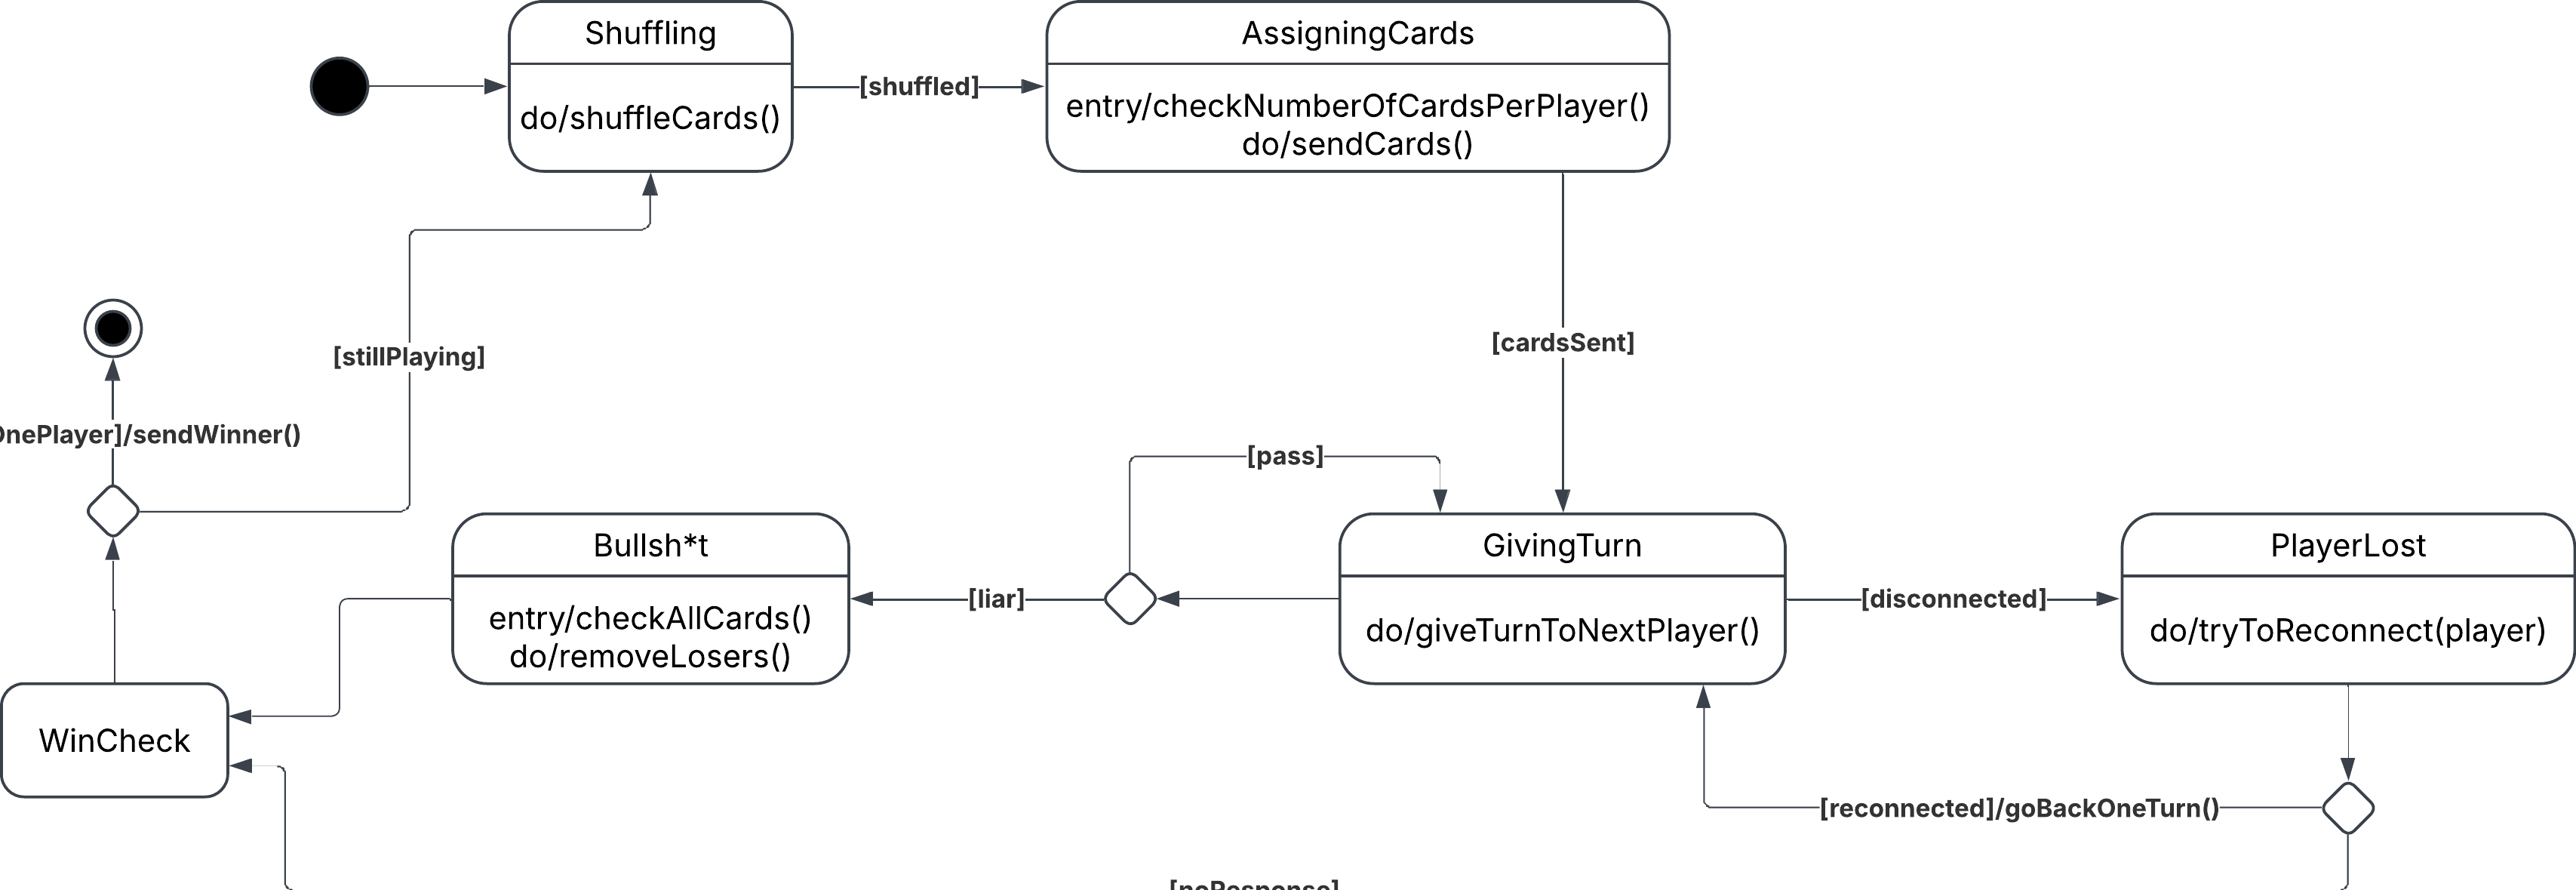
\includegraphics[width=0.8\textwidth]{figures/gameAgentStates.png}
                  \caption{State diagram of the game agent}
                  \label{fig:gameAgentStates}
            \end{figure}
\end{itemize}

\subsection{Data and Consistency Issues}\label{data-and-consistency-issues}
Since we don't need to store data permanently because this is a card game, we don't deal with queries
and databases.

Some data is shared between components, for example the game status, the players' nicknames, and
other crucial information to perform the game.

\subsection{Fault-Tolerance}\label{fault-tolerance}
Different types of fault tolerance are implemented in the systems, everything is set up to keep
the game running even if some components fail.

The mechanics differ in their scope and purpose:
\begin{itemize}
      \item
            \textbf{Server-Side} \par
            The server and the broker are at the core of the game, if they fail the game is lost.
            To prevent this from happening, they are constantly monitored.

            These share the same mechanism of fault-tolerance, redundancy and backup,
            but differ in implementation:

            \begin{itemize}
                  \item \textbf{Backup Server} \par
                        The server is backed up by a second server that runs as a server but is
                        not active; so it only listens to the messages sent by the clients and the
                        broker and keeps a copy of the game state.

                        If the main server fails, the backup server can take its place and resume
                        the communication between the clients and the broker. This mechanism has a
                        limitation since doesn't keep a record of ongoing games, simply placing
                        players back in lobbies. This happens because the game loop runs as a separate
                        agent launched by the main server, so if the main server fails during a game,
                        the game loop is lost too; in that case, all the players receive a message
                        that the game is over before being redirected to the lobby screen.

                        All of this will use a heartbeat mechanism, where the server sends a
                        heartbeat message to the backup every 2 seconds. If the backup does not
                        receive the heartbeat message within the fixed time, it assumes that
                        the main server has failed and takes his place elevating itself to the role of
                        main server.
                  \item \textbf{Broker Backup} \par
                        The broker is backed up by a second broker that keeps a copy of the messages
                        sent by the clients and the server.
                        If the main broker fails, the backup broker can take its place and resume
                        the communication between the clients and the server.
                        This will be using the mosquitto configuration file, where the main
                        server is configured to send a copy of every message to the backup broker
                        with a bridge connection.

                        The backup broker will be configured to listen to the same topics as the
                        main broker, so it can receive the messages sent by the clients and the server.

                        When the main broker fails, the \texttt{ConnectionHandler} class both used
                        by the client and server should try to connect to the backup broker,
                        and if it succeeds, it can resume all communications where they left off.
            \end{itemize}
      \item
            \textbf{Client-Side} \par
            To make sure that no accidental disconnection can ruin the game, the game agent gives to
            each player a minute to make a move, if the player does not respond in time, it will be
            kicked from the game, continuing with the remaining players.

            Nevertheless, if anything goes wrong the client always has the opportunity to try to
            reconnect, picking where it left off. While playing the web browser will save the user
            information in the local storage so that the client can retrieve it when trying to reconnect.
            If successful, the client will send a message to the server asking for the current game
            state, and the game agent will publish a message with the current game state.
\end{itemize}

\subsection{Availability}\label{availability}
We don't have any availability mechanism in our project.
We only use caching for the broker that keeps the last message sent in a topic
and the backup server that keeps a copy of the game state in case of failure.

\subsection{Security}\label{security}
There aren't any security mechanisms in our project.

\newpage
\section{Implementation}\label{implementation}
\subsection{Network Protocols}\label{network-protocols}
The main network protocol used is MQTT for the communication between the components.
To implement the MQTT protocol we used the Paho library for Python, which is a client library for 
the MQTT protocol.

Thanks to MQTT protocol and its path-like structure, we can easily create topics for each lobby 
and each player, allowing them to communicate with the server and with each other.

An example of a topic structure is:
\begin{itemize}
      \item \texttt{create\_lobby} for the lobby creation messages
      \item \texttt{join\_lobby} for players to join lobbies
      \item \texttt{lobby/}\textless LOBBY\_ID\textgreater\texttt{/raise\_stake} for the raise stake messages
      \item \texttt{lobby/}\textless LOBBY\_ID\textgreater\texttt{/check\_liar} for the liar detection messages
\end{itemize}

As we can see, the topics are structured in a way that allows us to easily identify the lobby and the 
type of message being sent. This is not always true, because all the messages sent before the lobby 
joining are sent to the general topic, so every player can see them, but after joining the lobby, the 
messages are sent to the specific lobby topic.

To recognize the messages in the general topic, we use a specific format for the messages, where the 
body contains the serialized player object. This part will be explained in more detail in the next 
sections.

The communication is done using a class called \texttt{ConnectionHandler}, which is responsible for 
managing the connection to the broker and the communication with the server. That class provides 
methods to subscribe to topics, publish messages, and handle incoming messages.

The clients are automatically subscribed to the game topics when they join a lobby, so they can 
receive the messages from the server. On the other hand, the server is subscribed to all the topics, 
so it can receive the messages from the clients and publish the game status.

This is the list of all the topics used in the system: (as said before, some topics are used directly 
in this way while others are used with a specific lobby ID and pattern):
\begin{itemize}
      \item \texttt{lobby}
      \item \texttt{new\_lobby}
      \item \texttt{new\_player}
      \item \texttt{ready\_to\_play}
      \item \texttt{start\_game}
      \item \texttt{join\_lobby}
      \item \texttt{leave\_lobby}
      \item \texttt{remove\_player}
      \item \texttt{start\_turn}
      \item \texttt{start\_round}
      \item \texttt{round\_loser}
      \item \texttt{game\_over}
      \item \texttt{raise\_stake}
      \item \texttt{check\_liar}
      \item \texttt{heartbeat}
      \item \texttt{server\_error}
      \item \texttt{game\_info}
\end{itemize}

\subsection{Data Formats and representations}\label{data-formats}
To make the communication between components through the MQTT protocol possible, a way to serialize
and deserialize the information in the form of messages is needed.
We decided to use JSON as the data format of choice, since it is lightweight and easy-to-use.
Through the use of the \texttt{json} library in Python, it was possible to create two classes used
by the connection handler to, respectively, serialize and deserialize the information:
\begin{itemize}
      \item \texttt{Serializer} is used to serialize the objects composing a Message dictionary into a 
            JSON string.
      \item \texttt{Deserializer} is used to deserialize the JSON string back into a Python
            object, which can be used by the application.
\end{itemize}

To implement these classes, we used as a starting point the code provided in the lab lessons with professor
\href{https://www.unibo.it/sitoweb/giovanni.ciatto}{Ciatto Giovanni}.

In short the message sent start as a Python dictionary of objects, then it gets serialized into a 
JSON string and sent to the broker, which then publishes it to the subscribed clients.
When a client receives a message, it deserializes the JSON string back into a Python dictionary, 
which can now be used to access the objects.

\subsection{Technological details}\label{technological-details}
The project is completely implemented in Python, using the following external libraries:
\begin{itemize}
      \item \href{https://pypi.org/project/paho-mqtt/}{paho-mqtt} is used to implement the MQTT 
            protocol and manage the communication between the components. This library provides a 
            simple and easy-to-use interface to connect to the broker, subscribe to topics, publish 
            messages, and handle incoming messages.
      \item \href{https://nicegui.io/}{nicegui} is used to implement the user interface of the game, 
            allowing players to interact with the game through a web browser. The strength of this 
            library is the ability to create both the interface and logic of the client as a single 
            Python script, which is then transformed into a single web application.
\end{itemize}

\newpage
\section{Validation}\label{validation}
\subsection{Automatic Testing}\label{automatic-testing}
For the automatic testing we used the \texttt{unittest} framework, which is a built-in Python module 
for testing code. Every component of the system is tested with a set of unit tests that check the 
functionality of the methods and the correctness of the data.
The command to run the tests is:
\begin{verbatim}
python -m unittest discover -s test -p '*_test.py'
\end{verbatim}

\begin{itemize}
      \item \textbf{Game}\par
            The game class is tested with different inputs and expected outputs, to ensure that the 
            game logic is correct. The tests check if the game can be started, if the players can be 
            added and removed, if the game can be played, and if the game can be ended. The tests also 
            check if the game state is correctly updated after each move.
      \item \textbf{Deck}\par
            The deck class is tested to ensure that the deck is correctly shuffled and that the cards 
            are correctly dealt to the players.
      \item \textbf{Stake}\par
            The stake class is tested to ensure that the stake is correctly raised and that the 
            minimum stake is correctly updated. The most complicated combinations of cards are tested 
            to ensure that the stake is correctly checked when raised and the next minimum stake is 
            correctly calculated.
      \item \textbf{Service}\par
            The service module is tested to ensure that it can correctly serialize and deserialize messages.
      \item \textbf{Connection}\par
            The connection module is tested to ensure that the connection to the broker is correctly 
            established and that the messages are correctly sent and received. The tests check if the 
            client can connect to the broker, if the client can subscribe to topics, if the client can 
            publish messages, and if the client can receive messages.
            Mosquitto is required to run the tests, so the command to run the tests is:
            \begin{verbatim}
mosquitto
python -m unittest test.services.connection.connection_handler_test
            \end{verbatim}

\end{itemize}

\subsection{Acceptance test}\label{acceptance-test}
To test the interaction between the components we used manual tests, for example, we created a 
lobby and joined it with multiple clients, then we tested the interaction between the clients and 
the server.
To run this type of test use the command:
\begin{itemize}
      \item Windows
            \begin{verbatim}
      .\start_test_game_ui.ps1 [number_of_clients] [d]
            \end{verbatim}
      \item Linux
            \begin{verbatim}
      ./start_test_game_ui.sh [number_of_clients] [d]
            \end{verbatim}
\end{itemize}
This will start the game with the specified number of clients, two mosquitto instances and two servers.
The clients connections are established from 127.0.0.1:8080 incrementing the port number for each 
client, so you can  open multiple clients in different browser tabs. More over, the \texttt{d} flag
is used to run the clients in debug mode, so you can see the logs in the console.

All the acceptance criteria were tested manually with these scripts and successfully passed.

We decided to not automatize this type of test because it requires a lot of interaction with the UI.

\newpage
\section{Release}\label{release}
The components are organized into a set of modules, each one with its own functionality.
As shown in \cref{fig:dependencyGraph}, all the modules depends on models classes, but every other 
module is independent of the others, so they can be used separately; in fact it is possible to run 
single components importing only the modules described below:
\begin{itemize}
      \item \textbf{Client}\par
            model, services and view
      \item \textbf{Server}\par
            model, controller
      \item \textbf{Broker}\par
            config
\end{itemize}
Eventually, it is possible to add the utils module to use debug and log features.

\begin{figure}
      \centering
      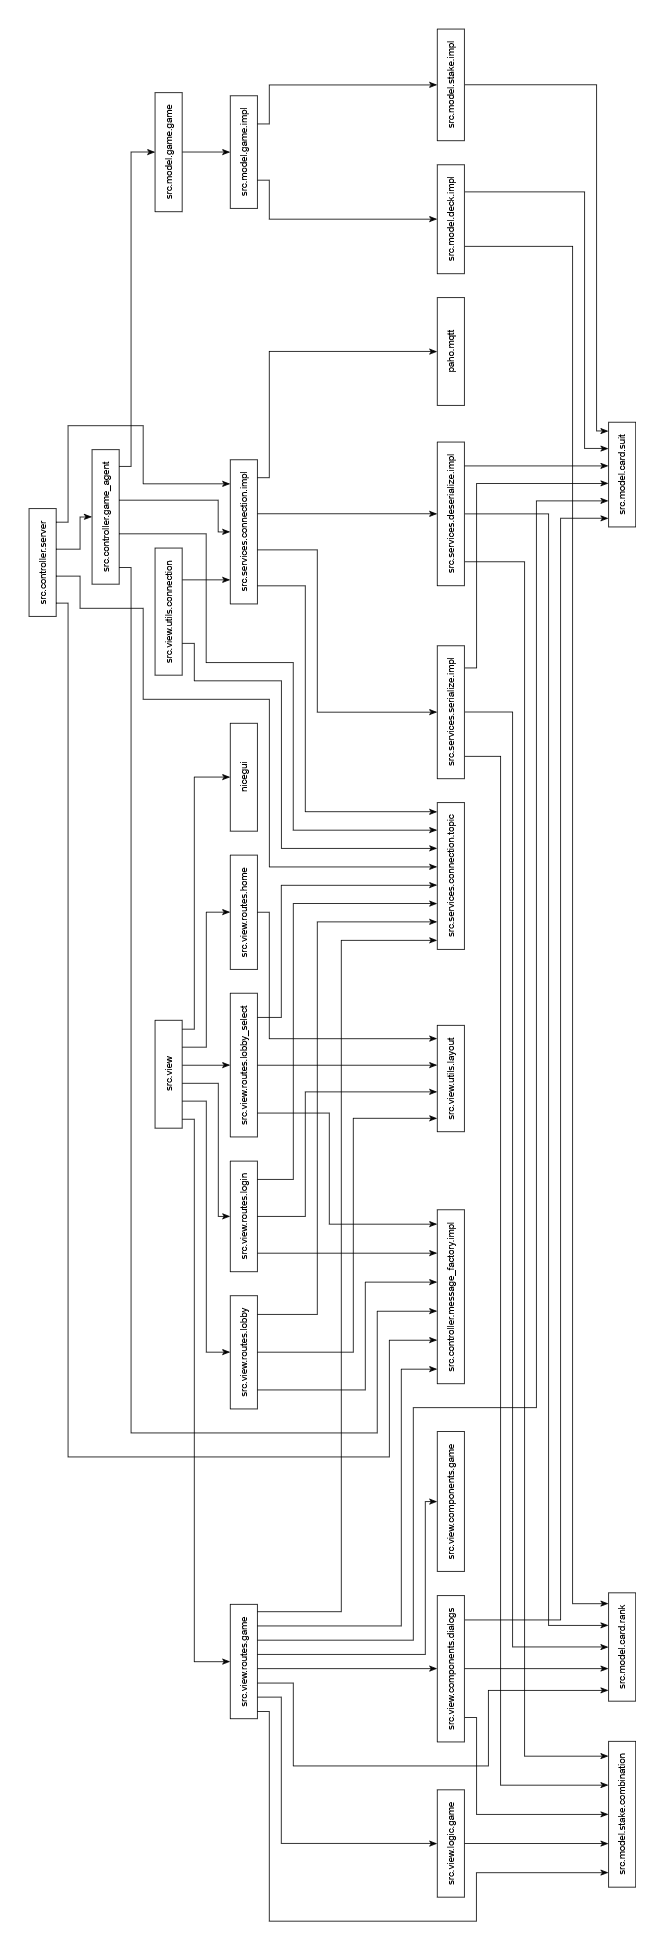
\includegraphics[width=0.5\textwidth]{figures/dependencyGraph.png}
      \caption{Dependency graph of the system}
      \label{fig:dependencyGraph}
\end{figure}

\newpage
\section{Deployment}\label{deployment}

The software is deployed on GitHub, where the source code is available. The repository is public, so 
anyone can access it. The repository is organized in a way that allows to easily navigate through the 
code and find the files needed to run the software.

To download the software, you can clone the repository using the following command:
\begin{verbatim}
git clone https://github.com/FrancescoBuda3/LiarsPoker
\end{verbatim}
or download the zip file from the \href{https://github.com/FrancescoBuda3/LiarsPoker}{repository page}. 

\newpage
\section{User Guide}\label{user-guide}
\subsection{Requirements}\label{user-guide-requirements}
There are some requirements to run the software, they are listed below:
\begin{itemize}
      \item Mosquitto broker installed (version 1.6.9)
            You can download it from the official website choosing the right version for your operating system: 
            \begin{itemize}
                  \item Windows: \url{https://mosquitto.org/files/binary/} 
                  \item Linux: \url{https://mosquitto.org/files/source/}
            \end{itemize}  
      \item Python installed (version 3.12 or higher)
            You can download it from the official website: \url{https://www.python.org/downloads/}
      \item Poetry installed (version 2.1.3)
            You can download it following the documentation from the official website: 
            \url{https://python-poetry.org/docs/#installation}
\end{itemize}

\subsection{Installation}\label{installation}
Since the project is developed using Python, there are no particular installation steps, but you 
have to install the dependencies using Poetry.

To install the dependencies, you have to run the following command in the project root directory:
\begin{verbatim}
poetry install
\end{verbatim}

\subsection{Running the software}\label{running-the-software}
To run the software, you have to run the following command in the project root directory 
(each command must be run in a different terminal):
\begin{itemize}
      \item Broker
            \begin{verbatim}
mosquitto -c ./config/mosquitto1.conf
mosquitto -c ./config/mosquitto2.conf
            \end{verbatim}
      \item Server
            \begin{verbatim}
poetry run python src/controller/server/__init__.py primary
poetry run python src/controller/server/__init__.py secondary
            \end{verbatim}
      \item Client
            \begin{verbatim}
poetry run python src/view/__init__.py [port]
            \end{verbatim}
\end{itemize}
To run the system in debug mode, you just have to add the \texttt{-d} flag at the end of each command.

\subsection{Screenshots}\label{screenshots}
Below are some screenshots of the software in action.

The application starts in the browser with the screen shown in \cref{fig:screenshot1}
and after pressing start you get redirected to the login screen \cref{fig:screenshot2}.

After logging in, the \cref{fig:screenshot3} shows the lobby selection screen, where the player can 
choose to create a new lobby or join an existing one. In \cref{fig:screenshot4} is shown the 
lobby screen, where the player can see the players in the lobby and set his status.

The other screenshots are related to the game:
\begin{itemize}
      \item \cref{fig:screenshot5} shows the in-game screen, where the player can see his cards, the 
            current player, the last stake and two buttons to raise the stake or call bullsh*t.
      \item \cref{fig:screenshot6} shows the dialog to choose the stake to raise.
      \item \cref{fig:screenshot7} shows the dialog with the hint of the possible combinations of 
            stakes
      \item \cref{fig:screenshot8} shows the dialog with the all the cards that were in game 
            when bullsh*t is called.
\end{itemize}

\begin{figure}
      \centering
      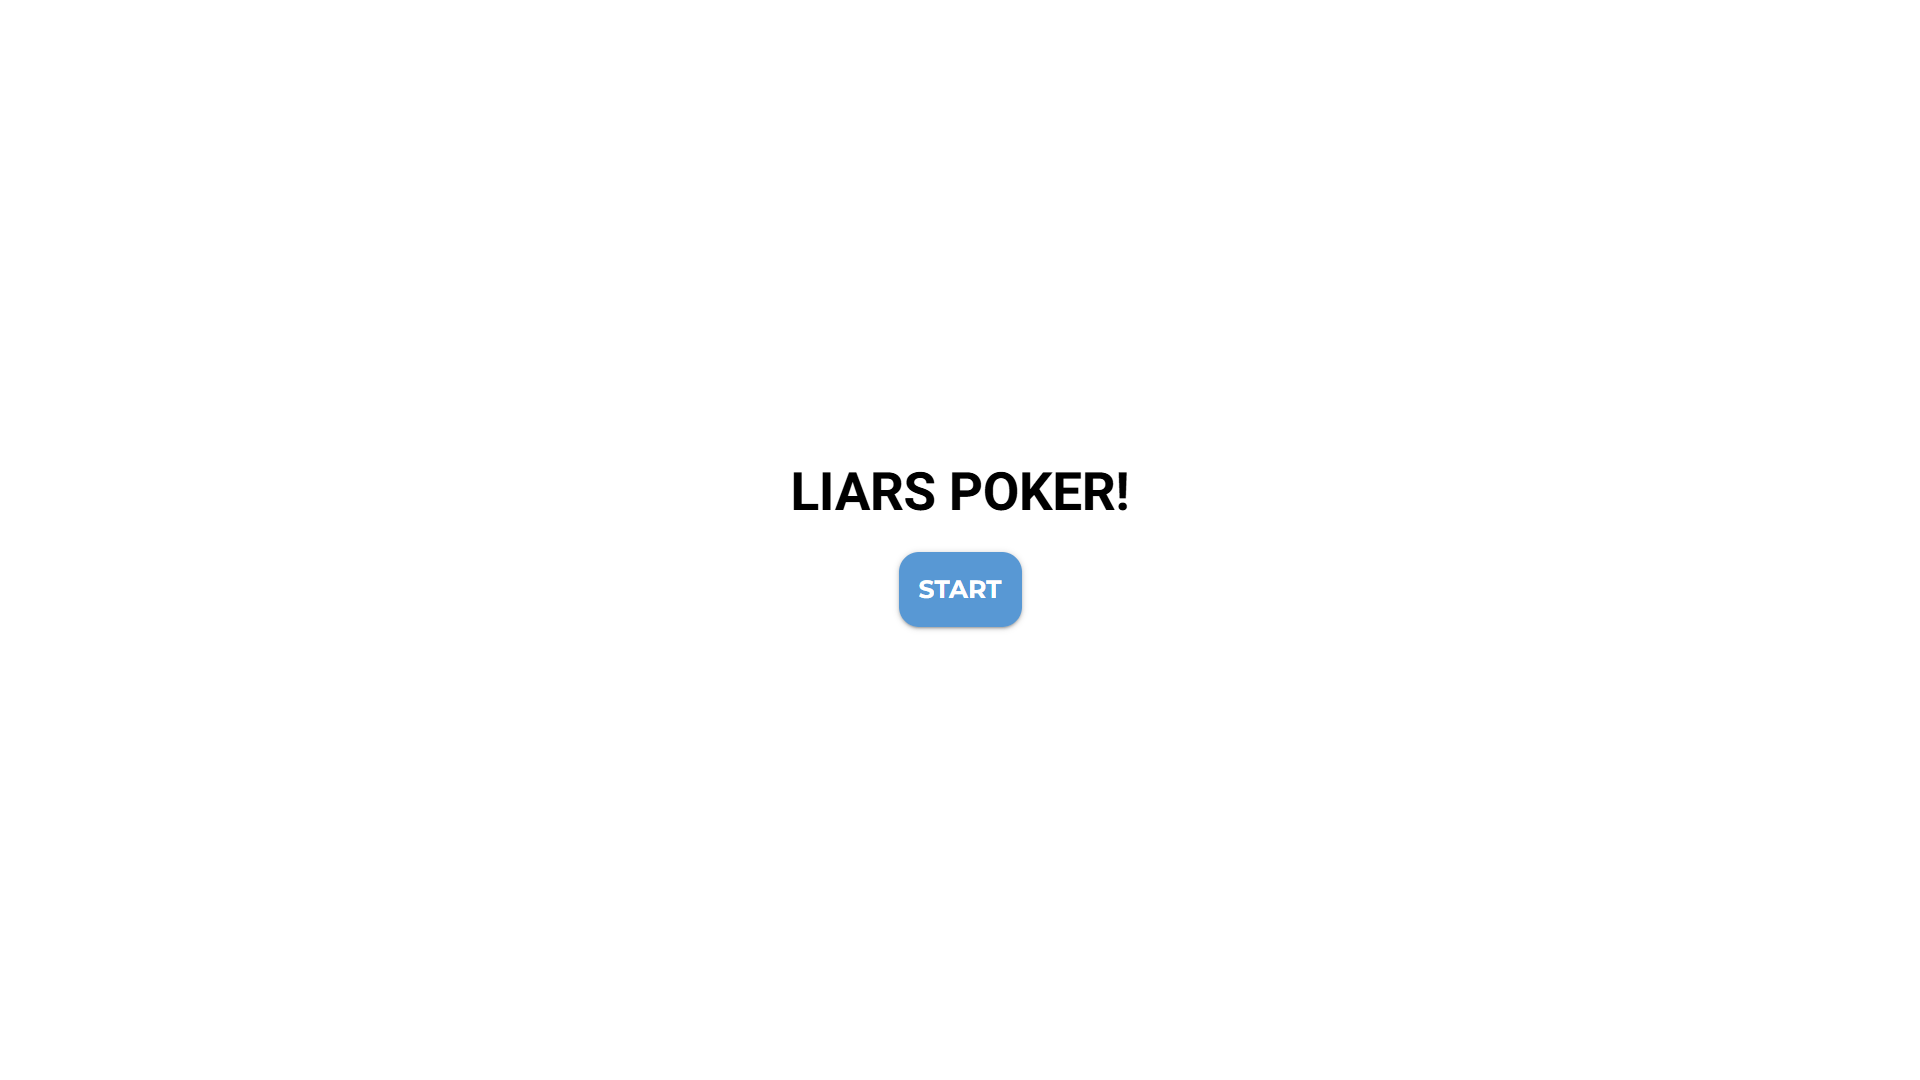
\includegraphics[width=0.8\textwidth]{figures/startupScreenshot.png}
      \caption{Screen after the startup}
      \label{fig:screenshot1}
\end{figure}

\begin{figure}
      \centering
      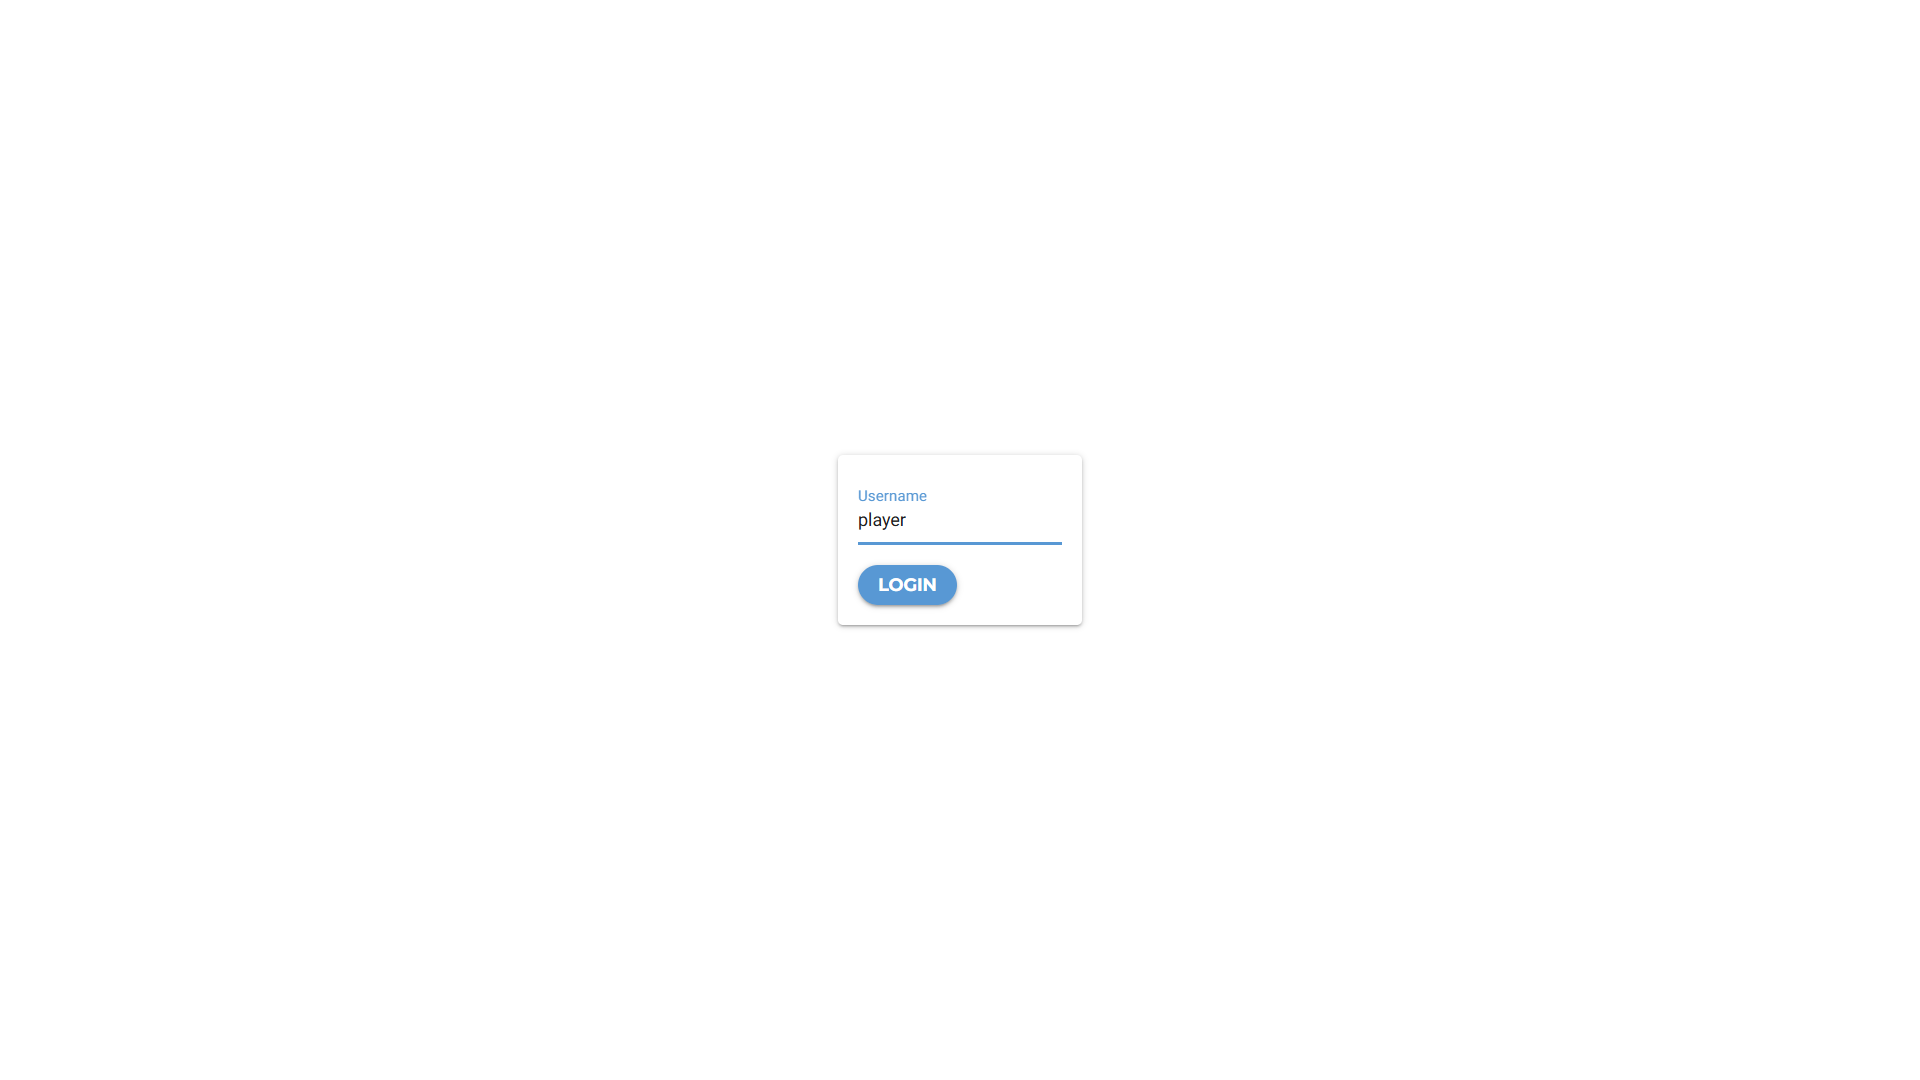
\includegraphics[width=0.8\textwidth]{figures/loginScreenshot.png}
      \caption{Screen to choose the nickname}
      \label{fig:screenshot2}
\end{figure}

\begin{figure}
      \centering
      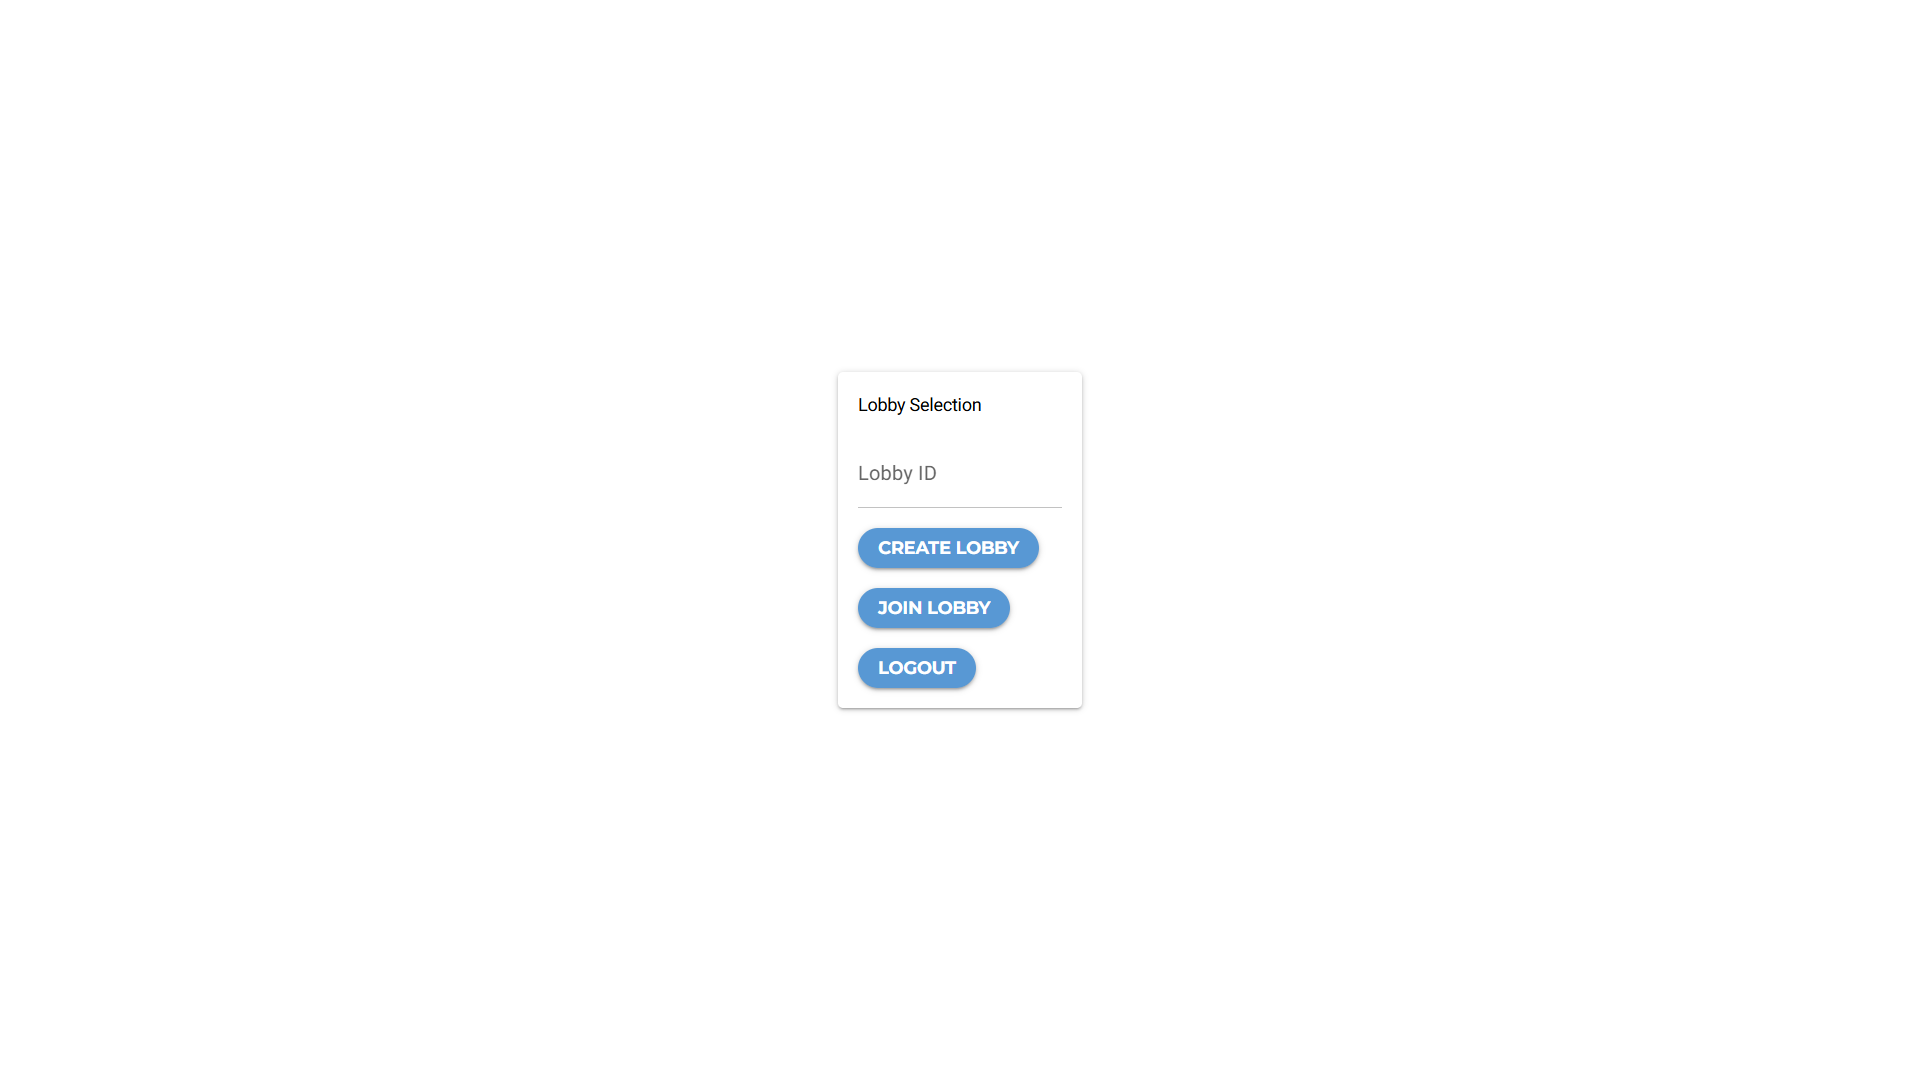
\includegraphics[width=0.8\textwidth]{figures/lobbySelectScreenshot.png}
      \caption{Lobby selection screen}
      \label{fig:screenshot3}
\end{figure}

\begin{figure}
      \centering
      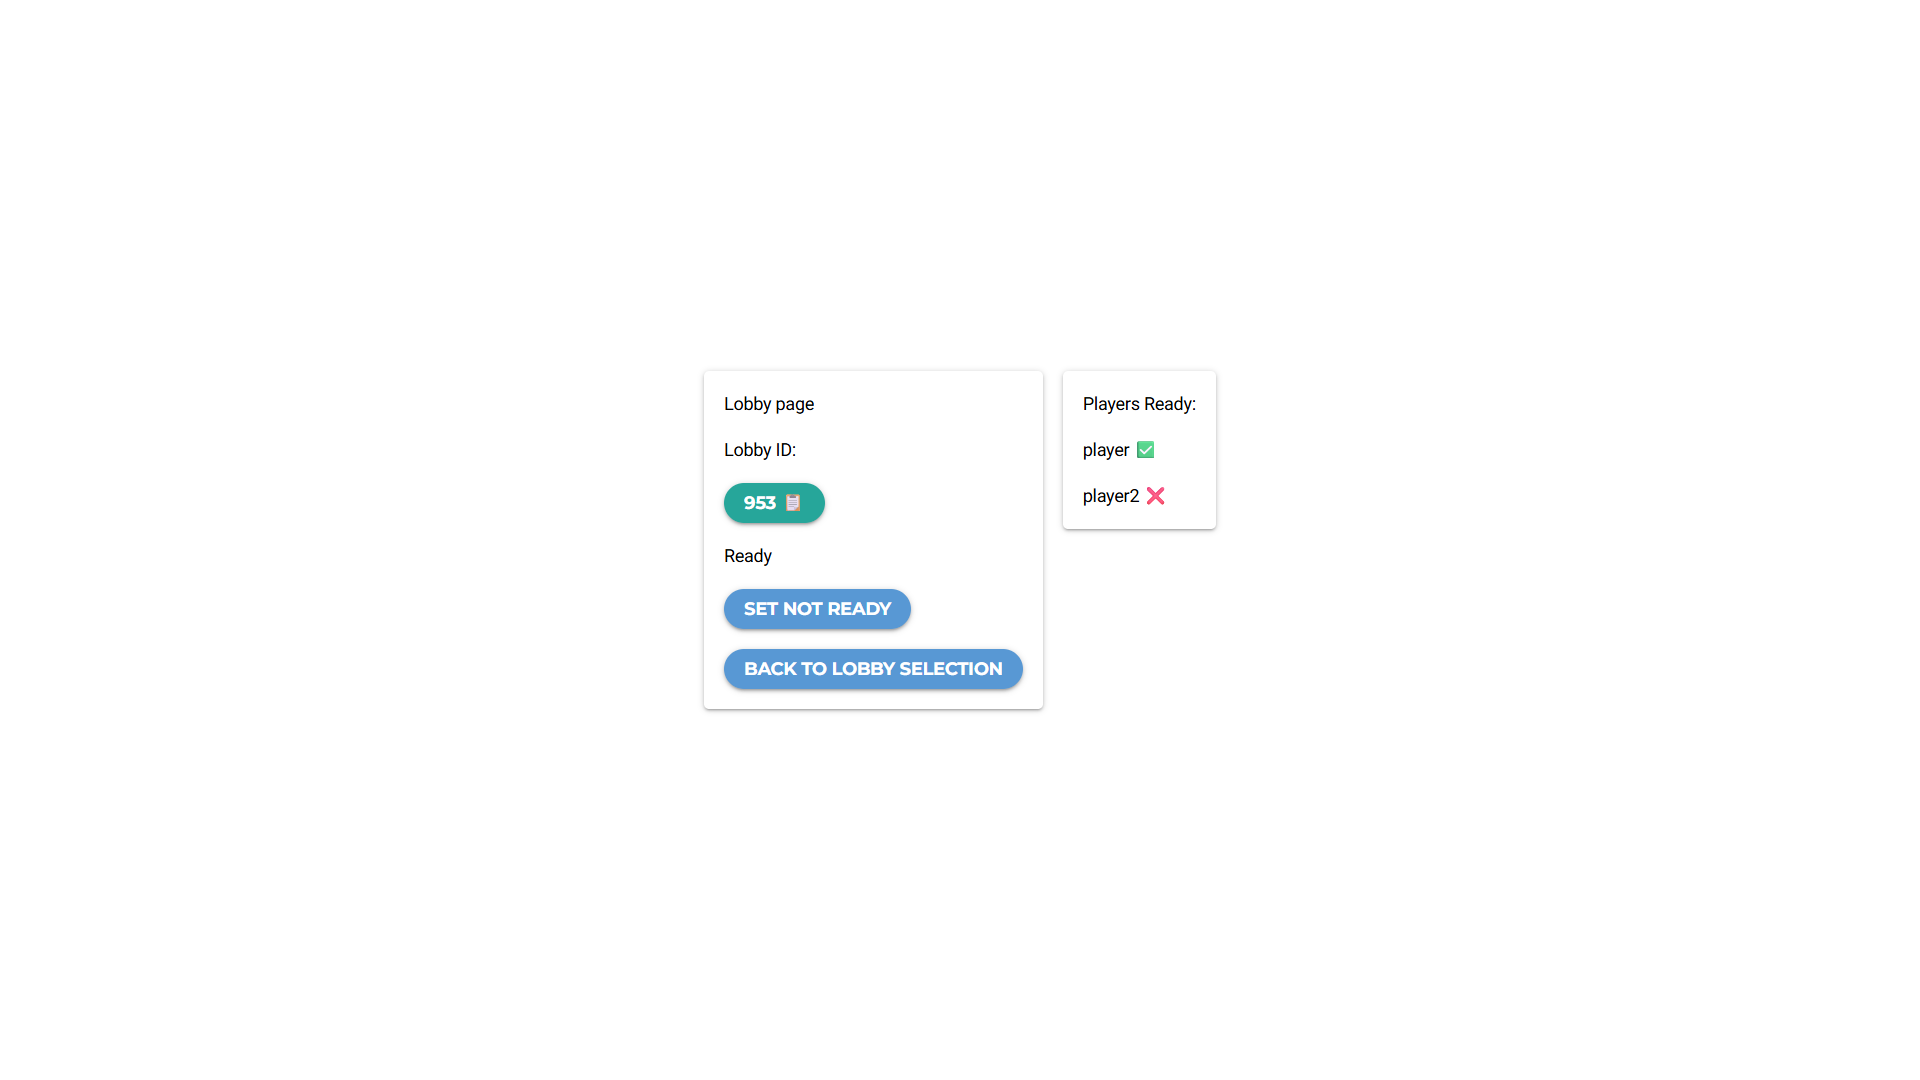
\includegraphics[width=0.8\textwidth]{figures/lobbyScreenshot.png}
      \caption{Lobby screen}
      \label{fig:screenshot4}
\end{figure}

\begin{figure}
      \centering
      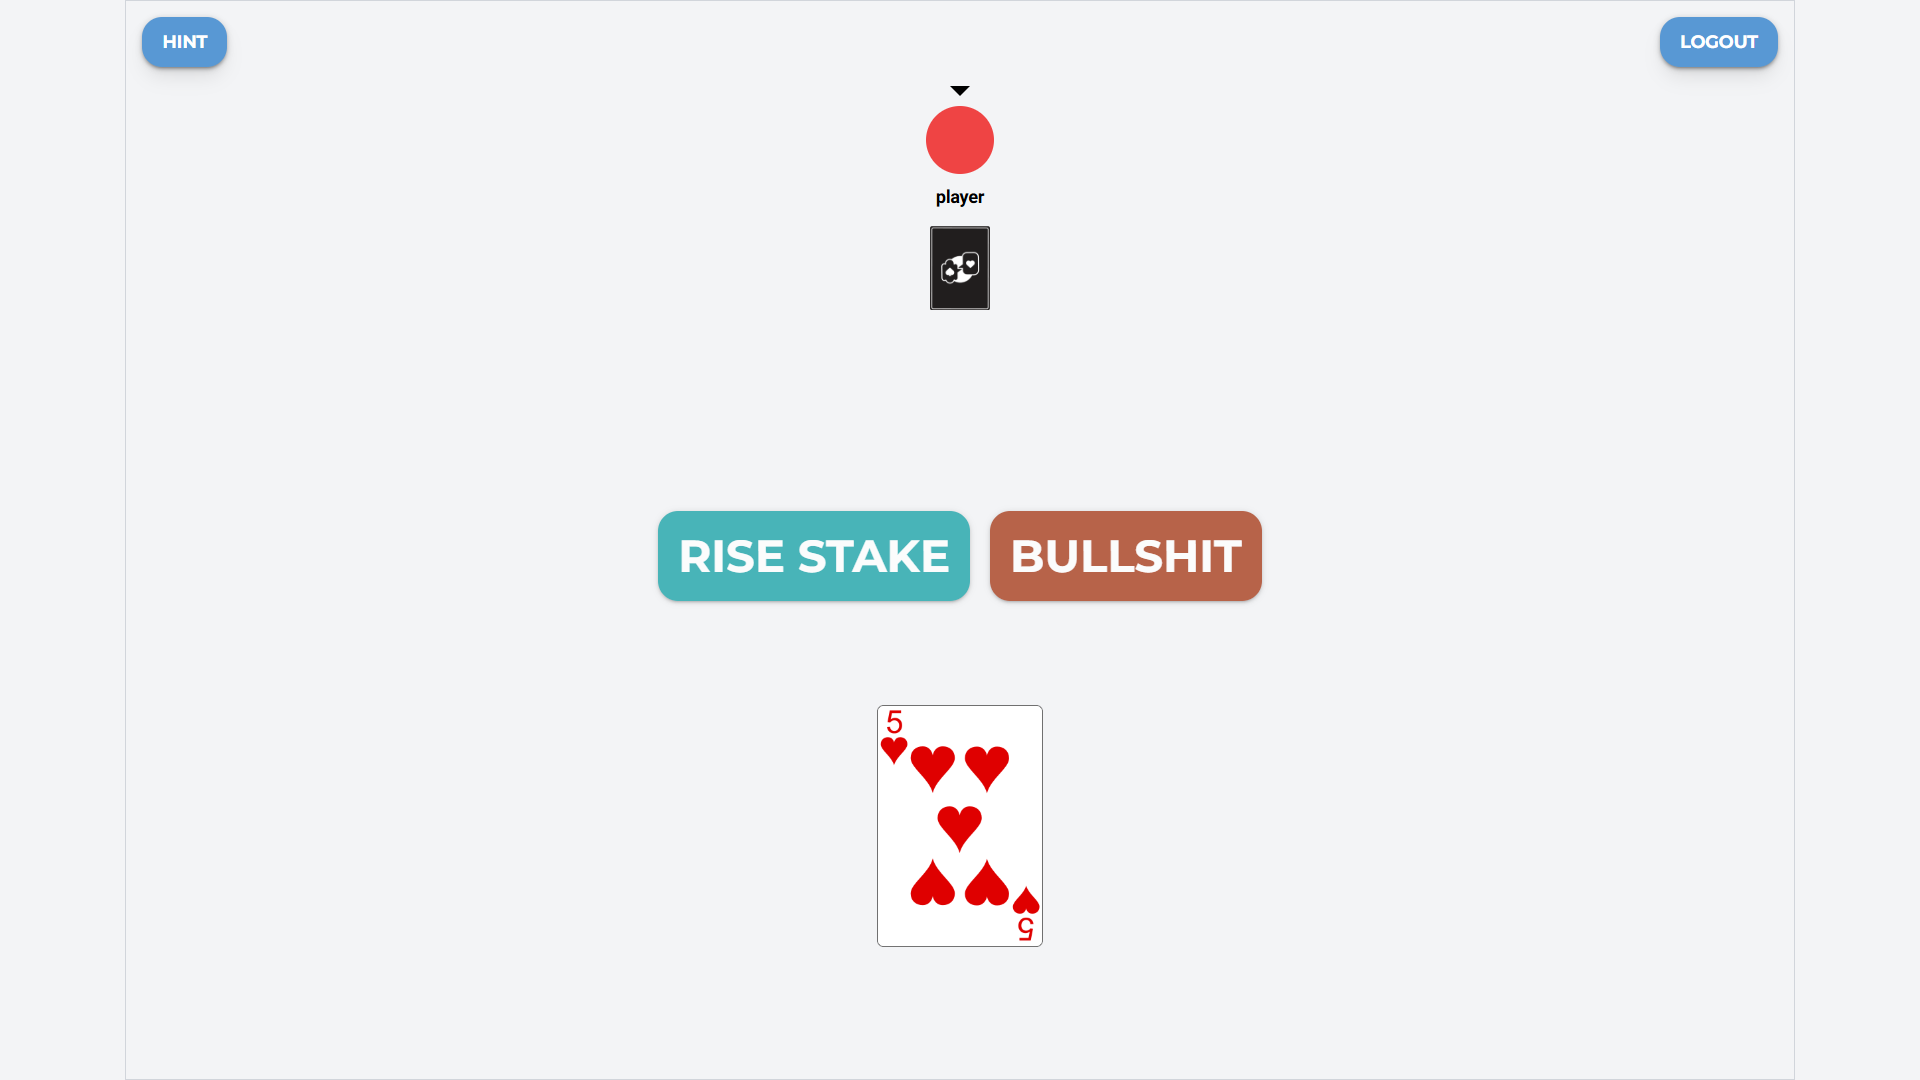
\includegraphics[width=0.8\textwidth]{figures/inGameScreenshot.png}
      \caption{In-game screen}
      \label{fig:screenshot5}
\end{figure}

\begin{figure}
      \centering
      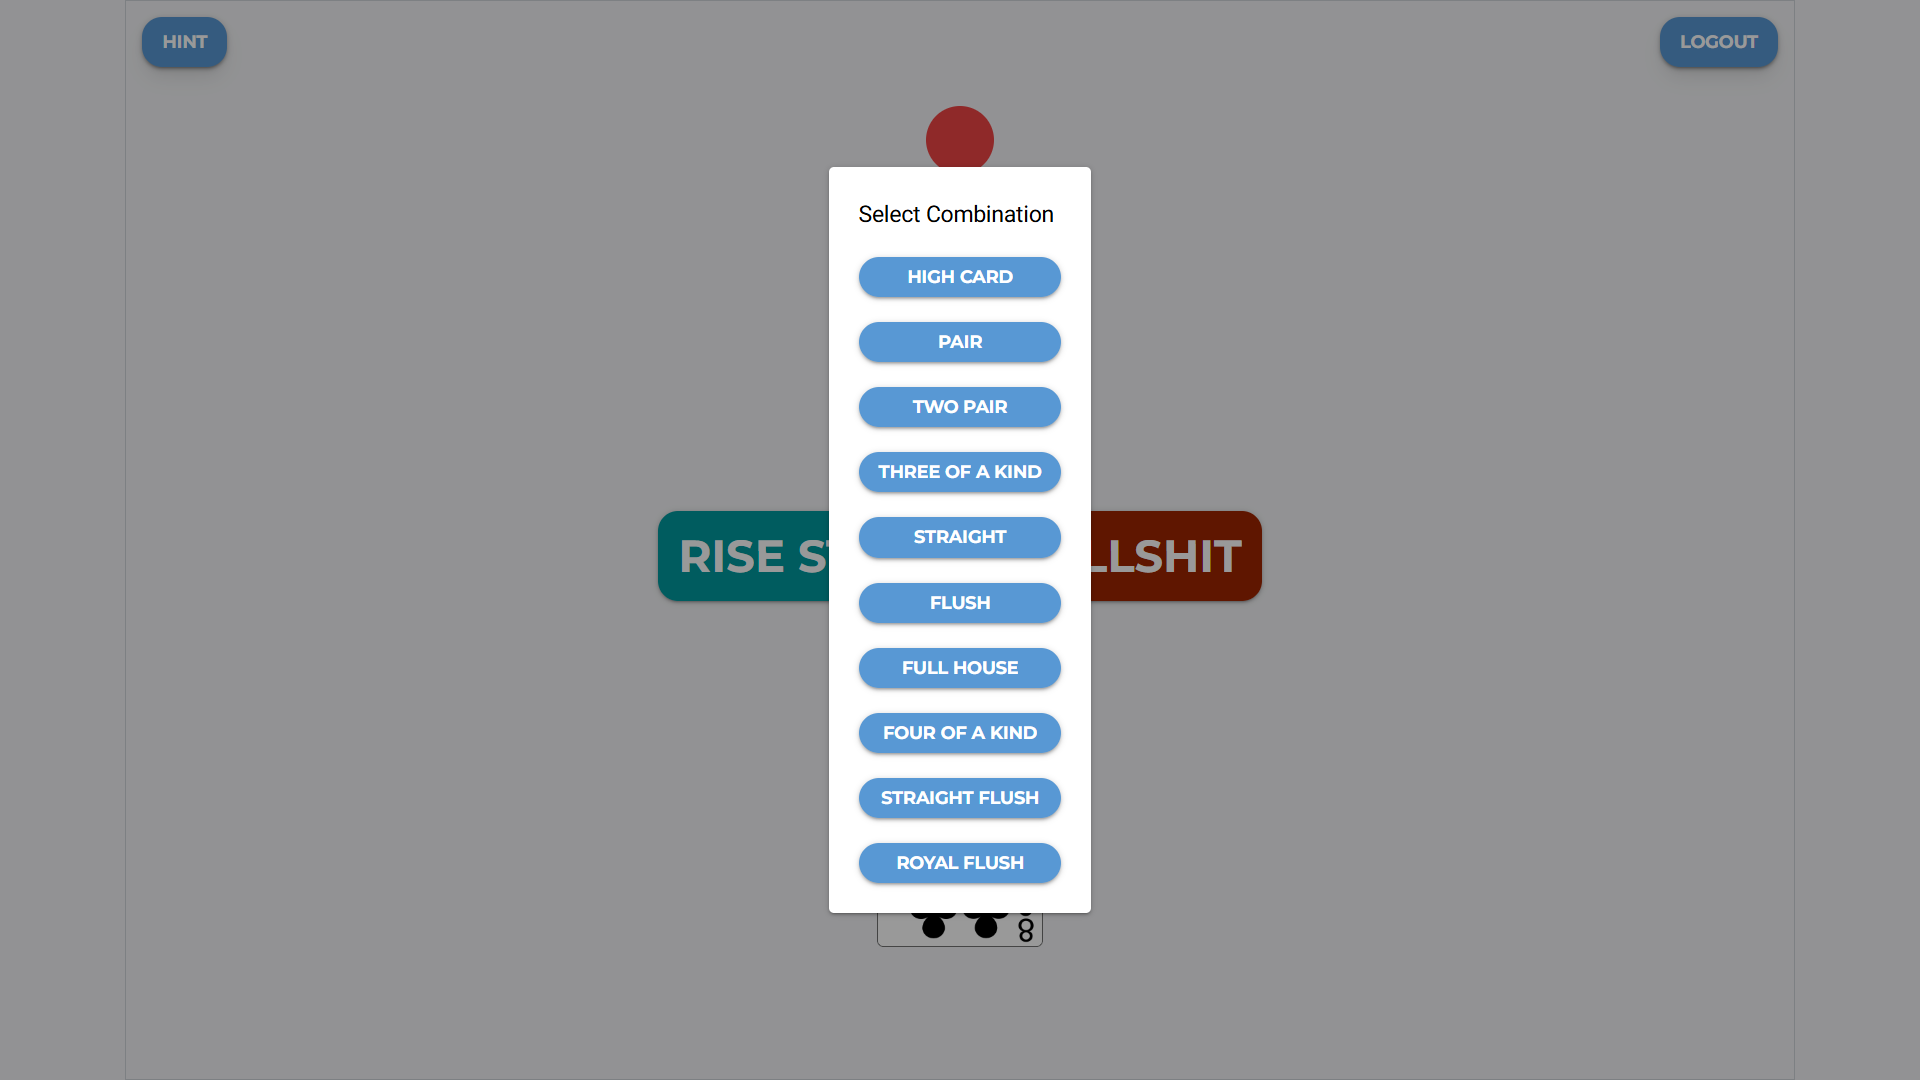
\includegraphics[width=0.8\textwidth]{figures/chooseStakeDialogScreenshot.png}
      \caption{Dialog to choose the stake}
      \label{fig:screenshot6}
\end{figure}

\begin{figure}
      \centering
      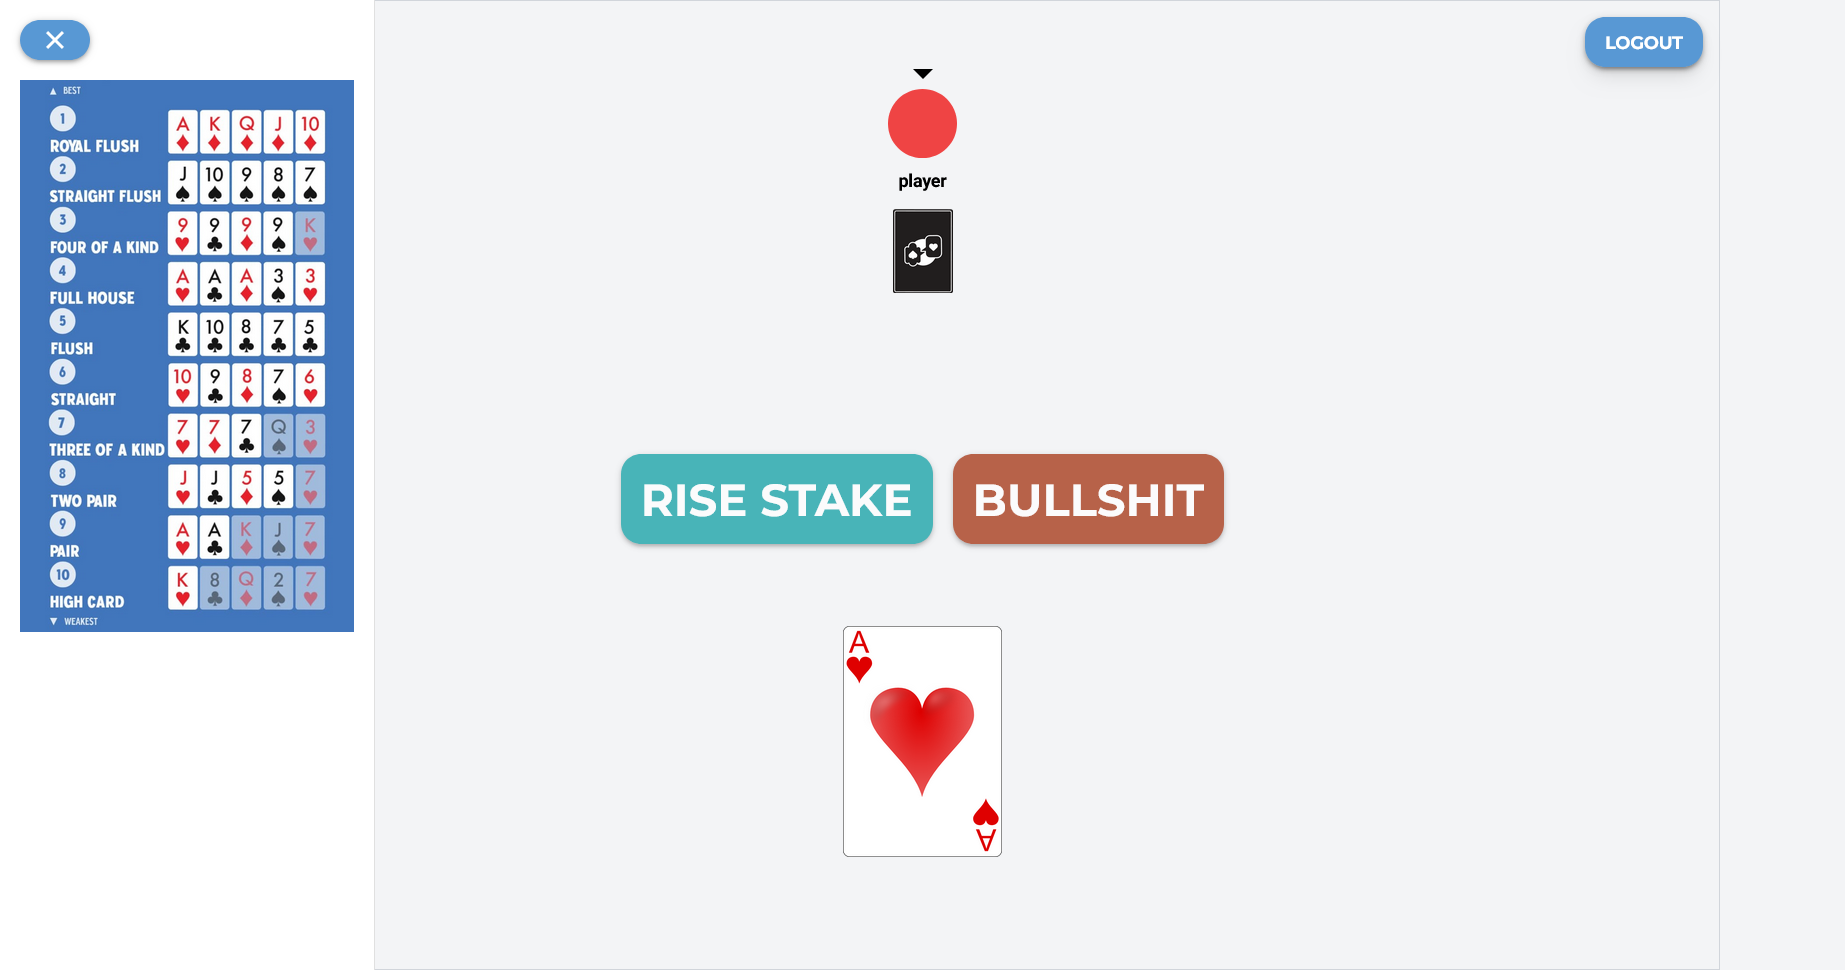
\includegraphics[width=0.8\textwidth]{figures/hintScreenshot.png}
      \caption{Dialog showing the hint for combinations}
      \label{fig:screenshot7}
\end{figure}

\begin{figure}
      \centering
      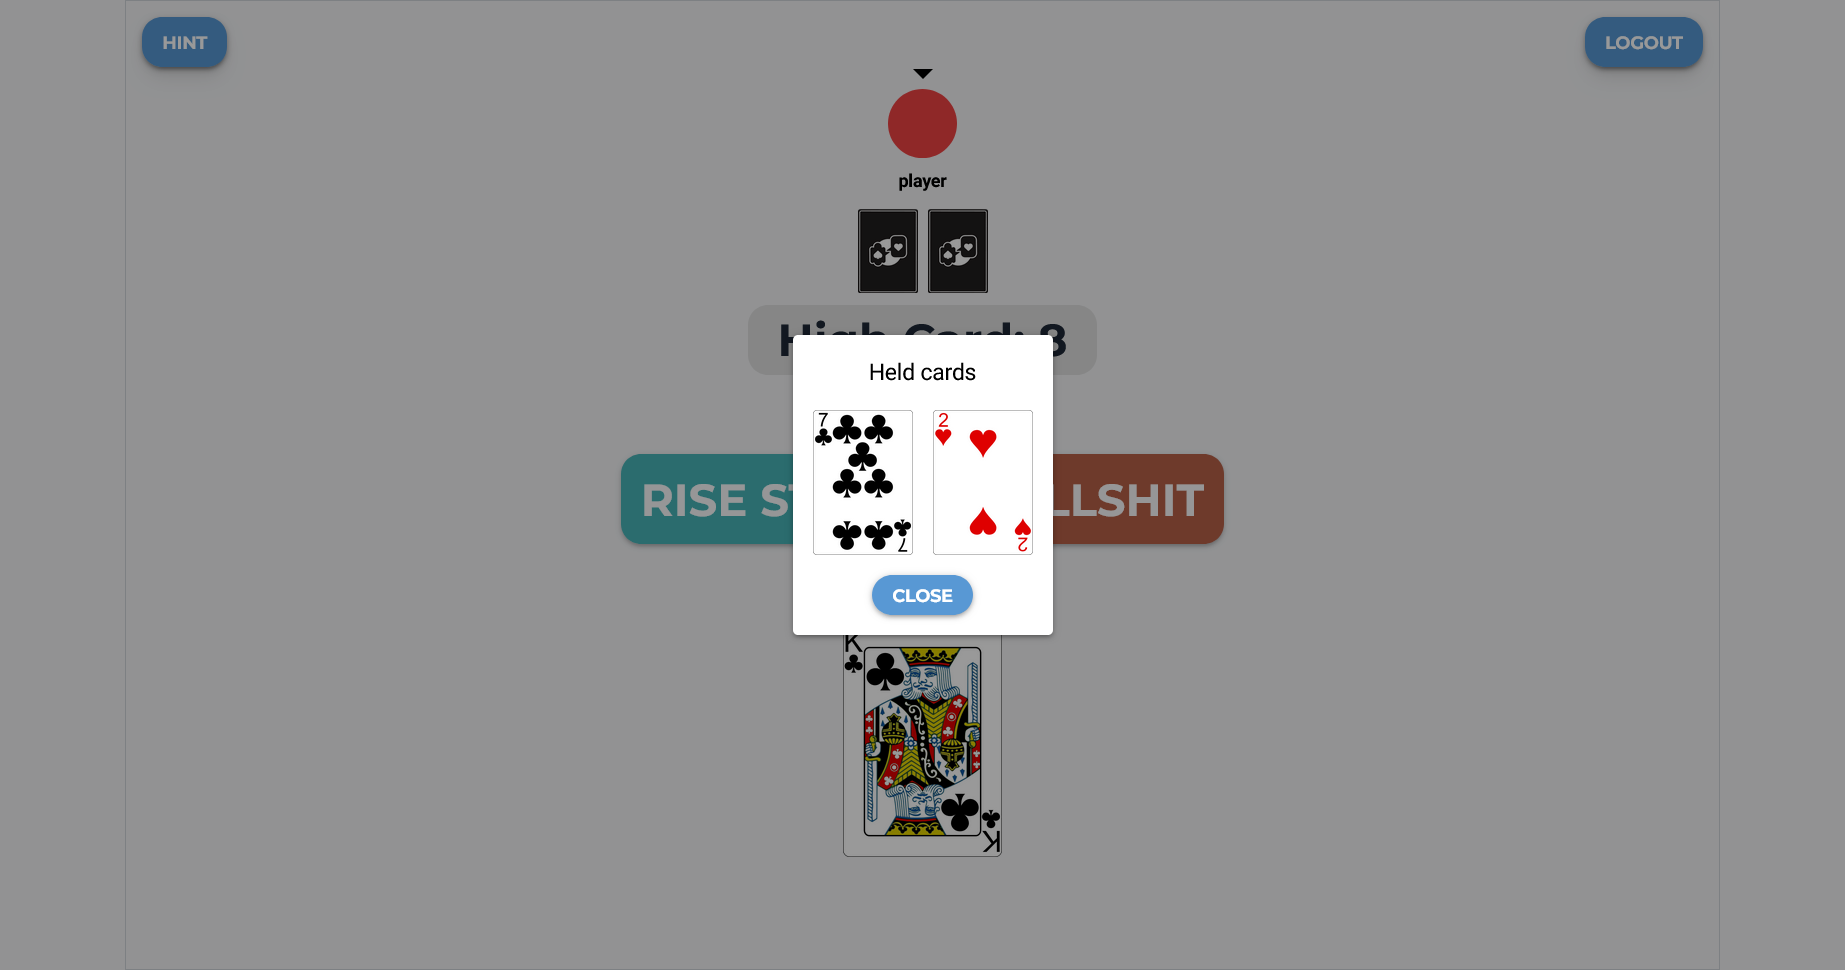
\includegraphics[width=0.8\textwidth]{figures/cardsInGameScreenshot.png}
      \caption{Dialog showing the cards in game after bullsh*t being called}
      \label{fig:screenshot8}
\end{figure}

\newpage
\section{Self-evaluation}\label{self-evaluation}
\subsection{Francesco Buda}\label{francesco-buda}
As a member of the group, my first role was to think about the requirements and use cases of the application,
considering also what we wanted the behaviour of the system to be in case of errors or unexpected situations.
I implemented the core game logic classes, in charge of managing the game state, and designed the related 
message structures. I also implemented the deserializer class, the connection handler class, which is
responsible for managing the message exchanging between the server and the clients, and the client-side fault
tolerance mechanisms.

I think the workflow of the project was well organized, also thanks to Tommaso Severi, who
was the one who kept the group together and made sure that everything was working as expected having a precise
overall view on the project. On my side, I personally gave my best to be as good as possible in all the situations
and I think the final product is a well-made project, with a good level of complexity and good code quality. 
As the design is, on my opinion, strong and well done, the weaknesses or improvements that could have been made are
mainly related to the technical side in order to improve the reliability, security and availability of the system.

\subsection{Emanuele Sanchi}\label{emanuele-sanchi}
My role in the group was to design the architecture of the system and to implement the server-side 
logic designing also the interactions between the components. I implemented the server-side classes, 
which are responsible for managing the game state and the players' actions, and I also implemented 
the fault tolerance mechanisms on the server-side (both for python server and for the MQTT broker). 
I also implemented much of the MessageFactory class methods; this class is responsible for creating 
the messages with a certain structure. In addition, I helped to create a base version of some 
client-side pages like the game page or the lobby selection page, to test my previous work like interaction 
with the server and with the other players. The final version of these pages were then implemented by 
the rest of the team. The weaknesses or improvements 
that could have been made are mainly related to the user experience, the security of the system which 
could be improved in future versions and the fault tolerance mechanisms that could be more robust for 
example by adding a database to store the game state and the players' actions. Overall, I am satisfied 
with the result and I think that the project is a good example of a distributed system.

\subsection{Tommaso Severi}\label{tommaso-severi}
I was in charge of designing the class and state diagrams of the system in the design phase, always
keeping an eye on the requirements and the architecture of the system during the whole process.
During the implementation I mainly occupied myself in the stake related logic and representation in the 
system, but also adapted the serializer class. I created the game-agent,
implemented the ready logic of lobbies in the server and further implemented the view modules.
My role in the group was to be the glue between the components, making sure that everything
was working together and that the system was coherent with the design.
I think that the final product has a high level of code quality, even with the restrictions of the
Python language, and the architecture is well-thought-out, allowing for easy maintenance and
future extensions. Despite that it surely could be polished adding more controls for corner 
cases and improving the user experience, overall I am more than satisfied with the result. I think 
that it is a great proof of concept, completely working, of a distributed system, with a good level of
complexity that shows the capabilities of the technologies used.

\bibliographystyle{plain}
\bibliography{references}

\end{document}
